\documentclass[pre,twocolumn,superscriptaddress,showpacs,floatfix]{revtex4-2}
\usepackage{amsmath,amssymb,bm}
\usepackage{graphicx}
\usepackage{xcolor}
\usepackage[colorlinks=true,linkcolor=blue!60!black,citecolor=blue!60!black,urlcolor=blue!60!black]{hyperref}

% Values still being measured (Phase 8) are marked so that none survives into a submission.
\newcommand{\pending}[1]{{\color{red}[#1]}}
\newcommand{\qs}{q^{*}}
\newcommand{\ds}{\mathrm{d}}

\begin{document}

\title{Discontinuous transition into two symmetric absorbing states in two dimensions}

\author{\pending{Author}}
\affiliation{\pending{Affiliation}}

\date{\today}

\begin{abstract}
In two dimensions, transitions from an active phase into one of two absorbing states related by a
$\mathbb{Z}_2$ symmetry are believed to be continuous, in the generalized voter class or split into
Ising and directed-percolation transitions, with mean-field bistability washed out by
fluctuations. We study stochastic cellular automata on the square lattice that interpolate
between an asynchronous, noisy Day \& Night rule and the voter model and have exactly two
absorbing configurations. Discontinuous transitions into symmetric absorbing \emph{phases} with
internal dynamics, and into three or more symmetric absorbing states, are known; for exactly two
absorbing configurations, the setting of the generalized voter theory, we report the first
transition that is fully first order, at every voter weight studied up to $p = 0.995$. Fronts
between the active and an absorbing phase reverse direction linearly at the transition point
$\qs$; the interface density stays finite down to $\qs$ and does not shrink with system size;
below $\qs$ the active phase is metastable and decays by nucleation and growth; above $\qs$ an
active droplet survives only beyond a critical radius that diverges at $\qs$; and the wall
between the two absorbing phases is wetted by an active layer whose thickness grows as $\qs$ is
approached. Near the voter point a parameter-free closure of the voter-model perturbation theory
predicts the transition line $\qs = c\,\alpha(1-p)$ with $c = 0.26\pm0.015$, against
$0.24$--$0.26$ in simulations, and suggests that the coexistence window closes only
logarithmically at the voter point. Applied to the five-cell automaton of Molofsky \emph{et al.},
where this regime was sought and not found, the closure predicts, and simulation confirms, a
transition line through its voter point, a metastable absorbing state in a band too narrow for
their search, and no metastable active phase.
\end{abstract}

\maketitle

%=====================================================================================
\section{Introduction}
\label{sec:intro}

Phase transitions into absorbing states are the best-studied class of nonequilibrium critical
phenomena~\cite{hinrichsen2000,odor2004,lubeck2004,henkel2008}. A system with a single absorbing
state and no further symmetry or conservation law generically belongs to the directed-percolation
(DP) class~\cite{janssen1981,grassberger1982}. Symmetry changes this. When the dynamics has two
absorbing states related by a $\mathbb{Z}_2$ symmetry, the one-dimensional transition belongs to
the parity-conserving (DP2) class~\cite{grassberger1984,menyhard1994,hinrichsen1997}, and in two
dimensions the generic case is the \emph{generalized voter} (GV) class~\cite{dornic2001}. The
voter model~\cite{clifford1973,holley1975,liggett1985} is its prototype: it has no surface
tension, coarsens with an interface density that decays only as $1/\ln
t$~\cite{cox1986,krapivsky1992,dornic2001}, and sits at the upper critical dimension
$d_c = 2$~\cite{janssen2005}. With three or more symmetric absorbing states the two-dimensional
transition is expected to be discontinuous, and a jump of the order parameter has been reported
for a three-state Potts-like model with absorbing states~\cite{lipowski2002,droz2003,azizi2018};
the two-state case is the one in which the voter class is expected to control the transition.

Al Hammal \emph{et al.}~\cite{alhammal2005} proposed a Langevin equation for this problem,
$\partial_t\phi = (a\phi - b\phi^3)(1-\phi^2) + D\nabla^2\phi + \sigma\sqrt{1-\phi^2}\,\eta$, with
the two absorbing states at $\phi = \pm 1$ and the disordered active state at $\phi = 0$. For
$b$ above a threshold the GV transition splits into an Ising transition and a DP
transition~\cite{droz2003,vazquez2008,azizi2020}. For $b<0$ mean-field theory gives a
discontinuous transition: the absorbing states remain linearly stable while a disordered active
state exists. In two dimensions, integrations of the equation at one noise strength led the
authors to expect a single GV transition, with ``fully first-order'' transitions only above two
dimensions~\cite{alhammal2005}. Castellano \emph{et al.}~\cite{castellano2009} gave the
mechanism: fluctuations carry the system from the active state over the mean-field barrier, but
not back. Simulations of microscopic two-dimensional models have since found GV behavior or an
Ising--DP split~\cite{dornic2001,droz2003,vazquez2008,castellano2009,lee2011,azizi2020}, and the
working hypothesis is that every $\mathbb{Z}_2$-symmetric absorbing transition in two dimensions
is of one of these two kinds.

That hypothesis has been tested on a narrow class of rules. In the lattice models listed, the
flip probability of a site is monotone, and nearly linear, in the number of disagreeing
neighbors, or the nonlinearity acts on the magnetization of a coarse-grained cell that is coupled
linearly to its neighbors~\cite{azizi2020}; and the noise is strong compared with the mean-field
barrier: Al Hammal \emph{et al.} integrated the Langevin equation in two dimensions at a single
noise strength, and Azizi and Pleimling reached $b = -8$~\cite{azizi2020} at a local noise
variance about twice the height of the deterministic barrier.
% Check: in the Langevin form of Azizi and Pleimling the noise variance is 2(1-phi^2), about 1.0
% at the barrier top of their potential at (a,b) = (-4.132,-8), whose height is about 0.44.
The Langevin equation that Vazquez and L\'opez~\cite{vazquez2008} derived from microscopic rules
keeps only the first derivatives of the flip probabilities, so it cannot see a bistability that
depends on their nonlinearity. Nothing excludes a discontinuous transition elsewhere, and none
of the arguments for washout is a theorem: the rigorous theory of voter-model
perturbations~\cite{cox2013,cox2025} establishes coexistence of an active phase with linearly
stable absorbing states in $d \ge 3$, and states no result about the order of the transition in
$d = 2$~\cite{cox2025,chatterjee2013}.

Discontinuous transitions into \emph{symmetric} absorbing states are not unknown, and the cases
on record delimit what is new here. In one dimension, Bagnoli, Boccara, and
Rechtman~\cite{bagnoli2001,bagnoli2005} located a first-order line between the two
$\mathbb{Z}_2$-related absorbing states of a totalistic cellular automaton from the hysteresis of
a regularized model, with the caveat that ordered states of a one-dimensional system are only
marginally stable~\cite{hinrichsen2000fo} (see also Ref.~\cite{bassler1996}). In two dimensions,
Lipowski and Droz~\cite{lipowski2002} found a jump of the active-site density for a Potts-like
model with \emph{three} absorbing states, confirmed by Azizi, Stidham, and
Pleimling~\cite{azizi2018}, who also showed that a twelve-neighbor version of the same model has
two continuous transitions instead. For the two-state version of that model Lipowski and Droz
called their results inconclusive, ``most likely'' first order~\cite{lipowski2002}; Droz,
Ferreira, and Lipowski~\cite{droz2003,droz2003b} then placed the nearest-neighbor model in the
voter class, found an Ising--DP split with twelve neighbors, and left the Moore-neighborhood
($z = 8$) case open as either voter-like or very weakly split. Rodrigues \emph{et
al.}~\cite{rodrigues2015} report a discontinuous line on small triangular lattices, but the
discontinuity is the jump of the magnetization that every voter-class transition has: because
the GV point has $\beta = 0$, it is itself often called first
order~\cite{deoliveira1993,dornic2001,vazquez2010}.

The closest precedents are the cyclic four-species models with site exchange of Szab\'o and
coworkers~\cite{szabo2004,szabo2005,szabo2007,szabo2007b,szabo2008} and of Guisoni, Loscar, and
Girardi~\cite{guisoni2013}. There, two ``defensive alliances'' of mutually neutral species are
absorbing in the sense that invasions stop inside them, the two alliances are related by a
symmetry, and the transition from the active four-species phase into an alliance is first order:
Szab\'o and Sznaider located it from the linearly vanishing invasion velocity of a planar
front~\cite{szabo2004}, the criterion we use below; above the threshold the two alliances coarsen
like an Ising model below $T_c$, separated by an active boundary layer~\cite{szabo2007}; and
with cyclic asymmetry the first-order lines end at a triple point or at directed-percolation
critical points~\cite{guisoni2013}. An alliance, however, is not a configuration but a set: any
mixture of its two species, exponentially many configurations, is absorbing, and the exchange
moves keep diffusing inside it. The Langevin description with absorbing boundaries at
$\phi = \pm1$ does not apply to such a phase, and no result for it bears on the generalized voter
class. The question left open by all of this work is the one the GV theory is about: can the
transition into \emph{exactly two} absorbing configurations be first order in two dimensions? We
answer it with the strict operational definition of the ``fully first-order'' transition of
Ref.~\cite{alhammal2005}: the order parameter of the active phase, its interface density, jumps
to zero at the transition, and the transition shows the hallmarks of phase
coexistence---stationary planar fronts, metastability, and nucleation.

The model we use belongs to the class of nonlinear voter models introduced by Cox and
Durrett~\cite{cox1991} and studied as synchronous cellular automata by Molofsky \emph{et
al.}~\cite{molofsky1999} and Schweitzer and Behera~\cite{schweitzer2009}: the flip probability
of a site depends only on the number of disagreeing neighbors, and the two uniform states are
absorbing. The question was in fact asked in that setting. The mean-field map of Molofsky
\emph{et al.} has a ``multiple outcome'' regime in which the symmetric active state and the two
absorbing states are all stable, and the authors searched for it in the two-dimensional automaton
with the five-cell neighborhood and did not find it: small seeds of the rare species nucleated the
active phase instead, and they concluded that the spatial model has no such
regime~\cite{molofsky1999}. Cox, Durrett, and Perkins~\cite{cox2013} later proved for $d\ge3$
that in this regime (their Case~4A) the active phase coexists with the linearly stable absorbing
states, winning by invasion. In $d = 2$ the case has remained open. We return to their
automaton in Appendix~\ref{app:molofsky}: simulated to within $10^{-4}$ of the transition line
that our closure predicts for it, it does show Case~4A, in a band $2\times10^{-3}$ wide in $p_1$ at
distance $0.05$ from the voter point, far below the resolution of their search; what it does not
show is a metastable active phase.

Discontinuous absorbing transitions with a unique absorbing state, or with non-symmetric ones,
are well established in two dimensions~\cite{ziff1986,bidaux1989,odor1996,lubeck2006,grassberger2006},
including in stochastic versions of the game of Life~\cite{schulman1978,monetti1995,monetti2001},
although low-dimensional fluctuations and quenched disorder tend to round
them~\cite{hinrichsen2000fo,villamartin2014}. For exactly two symmetric absorbing configurations
in two dimensions, no fully first-order transition has been reported.

Here we show that such a transition exists. We study a two-dimensional stochastic cellular
automaton built on the Day \& Night (D\&N) rule, a self-complementary Life-like
rule~\cite{eppstein2010}, made asynchronous and noisy, and mixed with the voter model with weight
$p$ (Sec.~\ref{sec:model}). Life-like rules under stochastic or $\alpha$-asynchronous updating
show both continuous transitions in the DP class~\cite{blok1999,fates2010} and first-order
ones~\cite{monetti1995,monetti2001,roy2024} between an active phase and an extinct or frozen one;
self-complementarity turns this single-absorbing-state problem into the $\mathbb{Z}_2$ problem.
For every $p>0$ the model has exactly two absorbing states, which we prove with a short counting
argument. At the representative point $p = 1/2$ we establish every signature of a discontinuous
transition (Sec.~\ref{sec:flagship}). The first-order line runs from the D\&N limit $p\to 0^+$ to
$p = 0.995$, within half a percent of the voter point, with no sign of a tricritical point, and
the first-order behavior survives asynchronous updating (Sec.~\ref{sec:line}). Near the voter
point a closure of the voter-model perturbation theory of Cox, Durrett, and
Perkins~\cite{cox2013}, built on coalescing random walks run for a finite time, predicts the
structure of the transition line exactly and its amplitude to within about ten percent with no
adjustable parameter, and explains why the first-order character fades only logarithmically as
$p\to 1$ (Sec.~\ref{sec:theory}); applied to the five-cell rule of Molofsky \emph{et al.}, it
locates a transition line that a direct simulation of their rule confirms, together with a
metastable absorbing state over a band an order of magnitude narrower than ours, but not the
metastable active phase it also predicts (Appendix~\ref{app:molofsky}). Section~\ref{sec:discussion} states what is new relative to
the precedents above, discusses how the model escapes the washout argument, and lists open
problems.

%=====================================================================================
\section{Model}
\label{sec:model}

\subsection{Definition}

Each site $i$ of an $L_x\times L_y$ square lattice with periodic boundaries carries a state
$\sigma_i\in\{0,1\}$. Let $j_i$ be the number of sites among the eight Moore neighbors of $i$
whose state differs from $\sigma_i$. In one time step every site is updated simultaneously and
flips with probability $w(j_i)$, independently of the others, where
\begin{equation}
w(j) = (1-p)\,\alpha\,R(j) + p\,\frac{j}{8} + q\,\delta_{j,2},
\label{eq:rule}
\end{equation}
with $R(j) = 1$ for $j\in\{3,6,7,8\}$ and $R(j) = 0$ otherwise. The first term is the D\&N rule
B3678/S34678: a dead site becomes alive if it has 3, 6, 7, or 8
live neighbors, and a live site survives if it has 3, 4, 6, 7, or 8. The rule is
self-complementary, so in terms of disagreeing neighbors a site flips if and only if
$j\in\{3,6,7,8\}$, whatever its state. With probability $\alpha$ a site applies this flip
($\alpha$-asynchronous updating~\cite{fates2005,blok1999}). The second term is the synchronous
voter model on the Moore neighborhood: with probability $p$ the site copies a randomly chosen
neighbor. Since $w$ depends on the configuration only through $j$, Eq.~\eqref{eq:rule} is a
synchronous nonlinear voter model~\cite{cox1991,molofsky1999,schweitzer2009} with a nonmonotone
rate. The third term is a minority flip: a site with exactly two disagreeing neighbors flips
with additional probability $q$. We fix $\alpha = 1/2$ unless stated otherwise and use $q$ as the
control parameter; $p$ moves the model from the D\&N limit ($p = 0$) to the voter model ($p = 1$).

Since $w(0) = 0$, the uniform states (all 0, all 1) are absorbing, and Eq.~\eqref{eq:rule} is
invariant under $\sigma\to 1-\sigma$. For small $q$ the system coarsens toward one of the
absorbing states. For larger $q$ the minority flips keep interfaces dense, and the system settles
in a disordered active phase with finite interface density and zero magnetization.

\begin{figure*}
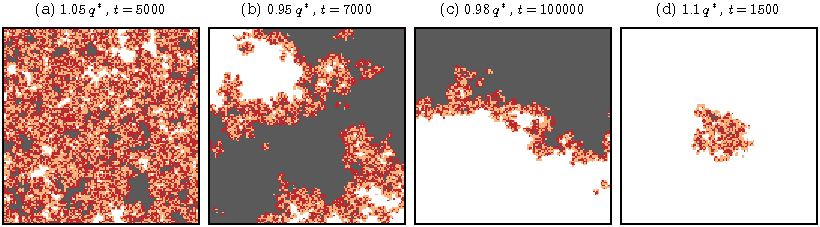
\includegraphics[width=\textwidth]{figs/fig_snap}
\caption{Configurations at $p = \alpha = 1/2$ ($\qs = 0.0459$). Sites without a disagreeing Moore
neighbor are white (dead) or gray (alive); sites with at least one are orange (dead) or red
(alive). (a) The active phase, $q = 1.05\,\qs$, $t = 5000$, $L = 256$. (b) Decay of the metastable
active phase by nucleation and growth of the two absorbing phases, $q = 0.95\,\qs$, $t = 7000$
($256^2$ window of $L = 512$). (c) A wall between the two absorbing phases, wetted by a layer of the
active phase, $q = 0.98\,\qs$, $t = 10^5$. (d) A supercritical droplet, $q = 1.1\,\qs$, $t = 1500$,
grown from a disordered disk of radius 20.}
\label{fig:snap}
\end{figure*}

\subsection{Exactly two absorbing states}
\label{sec:lemma}

A configuration is absorbing when no site can flip, i.e., when $w(j_i) = 0$ for all $i$.

\textit{Lemma.} On the square lattice with the Moore neighborhood, every rule with $w(j)>0$ for
all $j\in\{3,\dots,8\}$ has exactly two absorbing configurations, the two uniform ones,
whatever the values of $w(1)$ and $w(2)$.

\textit{Proof.} A nonuniform configuration contains two nearest neighbors $x$ and $y$ (sharing an
edge) in different states. They disagree with each other, and they share four further Moore
neighbors, each of which disagrees with exactly one of them. Hence $j_x + j_y \ge 2 + 4 = 6$, so
$j_x\ge 3$ or $j_y\ge 3$, and that site flips with positive probability. $\square$

For $p>0$, Eq.~\eqref{eq:rule} gives $w(j)\ge pj/8>0$ for every $j\ge 1$, so the lemma applies.
Moreover, since also $w(j)<1$, every configuration of a finite lattice reaches consensus with
positive probability (by repeatedly flipping only the boundary sites of the live clusters), so
the two uniform states are the only recurrent ones.
At $p = 0$ the lemma fails only through $w(4) = w(5) = 0$, and it fails badly: every
configuration in which all sites have $j\in\{0,1,4,5\}$ is frozen. These include the two
checkerboards and the diagonal stripe patterns of width two, and their number grows
exponentially with the area (Appendix~\ref{app:frozen}). They have no basin of attraction: a
single defect destroys them, and random initial conditions never end in them for $q>0$. Still,
they make ``two absorbing states'' false at $p = 0$, and we present $p = 0$ only as the limit
$p\to 0^+$ of the family. Appendix~\ref{app:frozen} also shows that regularizing the $p = 0$
rule directly, by a small flip probability $\epsilon$ at $j\in\{1,4,5\}$, moves $\qs$
continuously.

\subsection{Monotonicity and mean-field theory}
\label{sec:mf}

The model is attractive (monotone) when $w(j)$ is nondecreasing in $j$ and $w(j)+w(8-j)\le 1$,
because a site's probability of being alive after an update then increases with the set of live
sites. The second condition holds for $q\le(1-\alpha)(1-p)$, which covers all the $q$ studied
here. The D\&N term breaks the first at $j = 3\to 4$; the voter term restores it when
$(1-p)\alpha \le p/8$, i.e., for $p\ge 8\alpha/(1+8\alpha) = 0.8$ at $\alpha = 1/2$. The model is therefore nonmonotone for
$p<0.8$ and monotone above. None of our arguments uses monotonicity; we note it because the
first-order line extends into the monotone region, so nonmonotonicity is not what makes the
transition discontinuous. Monotone nonlinear voter models with two absorbing states and a
noise-free active phase in two dimensions are known, the threshold voter
models~\cite{liggett1994}; what is at issue here is the order of the transition, not the
existence of an active phase.

At the level of a pair approximation on the Bethe lattice with $z = 8$ (Appendix~\ref{app:pa}),
the absorbing states are linearly stable for every $p<1$ and the disordered active state is
stable as well, for every $q\ge 0$. The approximation is bistable everywhere and does not single
out a transition point: in a spatial system the phase is selected by which phase invades the
other. Mean-field bistability is precisely the situation in which washout is expected in two
dimensions~\cite{castellano2009}. Whether the two-dimensional transition is discontinuous is
therefore a question about fronts and fluctuations, and it is the question the simulations
address.

\subsection{Observables}

We measure the density $\rho$ of disagreeing nearest-neighbor bonds (the interface density per
bond), the fraction $\iota$ of sites with at least one disagreeing Moore neighbor, and the
magnetization $m = 2n-1$, where $n$ is the fraction of live sites. In the active phase
$\rho\approx 0.2$--$0.4$ and $m$ fluctuates around zero; in an absorbing phase $\rho = \iota = 0$.
The interface density is the order parameter. A transition is \emph{first order} in the sense
used here if (i) $\rho$ in the active phase stays finite as $q\to\qs{}^+$, independently of
system size, and (ii) the transition shows phase coexistence: a planar front between the active
phase and an absorbing phase is stationary at $\qs$ and moves with a velocity that changes sign
linearly there, the active phase is metastable below $\qs$, and an active droplet needs a finite
critical size to survive above $\qs$. At a GV point, instead, $\rho$ decays as $1/\ln t$ at
$q_c$; at a DP or Ising-type transition it vanishes continuously.

%=====================================================================================
\section{Methods}
\label{sec:methods}

\textit{Simulation.} We use a bit-parallel implementation in which each 64-bit word holds 64
sites and the neighbor counts and flip decisions are computed with bitwise operations. Each site
draws one uniform random number per step and flips if it is below the flip probability of its
class $(\sigma_i, j_i)$; all classes of a word share one bit-serial comparison, so the cost does
not depend on the number of distinct flip probabilities. Random numbers come from the
counter-based Philox$4\times 32$-10 generator~\cite{salmon2011}, keyed by the run's seed and
indexed by (time, row, word), so every run is bit-for-bit reproducible independently of the
number of threads and of restarts from checkpoints. The code passes a bit-exact comparison with a
naive per-site implementation for several rules and lattice shapes, and statistical tests of
the per-class flip frequencies (Appendix~\ref{app:numerics}). Near the transition it performs
about $10^9$ site updates per second per core.

\textit{Protocols.} We use five kinds of runs.
(i) \emph{Bulk}: random initial condition with density $1/2$ on an $L\times L$ torus.
(ii) \emph{Strip fronts}: on an $L_x\times L_y$ torus, the rows $y<L_y/2$ start random and the
rest dead, giving two flat fronts between the active phase and the absorbing state. The per-row
interface counts are recorded, each front is located where the smoothed profile falls below half
the interior value, and the velocity $v$ is the slope of the strip width, $W(t) = W_0 + 2vt$,
fitted while the interior is still active.
(iii) \emph{Tilted bands}: a band of direction $(a,b)$, the sites with
$(a y - b x)\bmod L < L/2$, on an $L\times L$ torus. Its two edges have total length
$2L\sqrt{a^2+b^2}$, and the normal velocity follows from the rate of change of the number of
interface cells, $\ds I/\ds t = 2L\sqrt{a^2+b^2}\,\iota_{\rm in}\,v$, with $\iota_{\rm in}$ the
interface fraction of the active interior.
(iv) \emph{Droplets and seeds}: a disk of radius $R$ whose sites are alive with probability $1/2$
(or a $2\times 2$ block of live sites) in the all-dead state. Many independent replicas are run;
since a site with $j = 0$ never flips, only the bounding box of the active region needs to be
updated, which is exact and makes each replica cheap. A replica that reaches the edge of the
lattice is counted as surviving.
(v) \emph{Walls}: all-alive rows $y<L_y/2$ and all-dead rows above, i.e., two flat walls between
the two absorbing phases and no active phase at $t = 0$.
Times are in steps (one synchronous update of all sites). Error bars are standard errors over
independent runs unless stated otherwise.

%=====================================================================================
\section{The transition at $p = 1/2$}
\label{sec:flagship}

We first establish the discontinuity at $p = 1/2$, roughly midway between the D\&N limit and the
voter point, where the model is nonmonotone, the transition line is near its maximum, and the
voter model's logarithms play no role. Figure~\ref{fig:snap} shows typical configurations.

\subsection{Fronts and their orientation}
\label{sec:fronts}

A strip of the active phase next to the absorbing state grows for $q>\qs$ and shrinks for
$q<\qs$, and the front velocity changes sign linearly at $\qs = 0.04596\pm0.00005$, with slope
$\qs\,\ds v/\ds q\approx 0.21$ (Table~\ref{tab:line}). Behind a retreating front the interior keeps
the interface-site fraction of the active phase ($\iota_{\rm in} = 0.71$ at $q = 0.95\,\qs$ against
0.76 at $\qs$), so the active phase is invaded at constant speed rather than decaying from within.
At a continuous transition the active density would instead vanish at $q_c$ and no retreating
front would exist below it. The linear reversal of a planar front is the criterion by which
Szab\'o and Sznaider located the first-order transition of the four-species alliance
model~\cite{szabo2004}, and it is how the winner of a bistable competition is decided in the
theory of spatial models~\cite{durrett1994,durrett2009}.

In nonequilibrium systems a stationary planar front does not by itself locate a transition: the
equistability point can depend on the orientation of the front, and between the extreme values a
finite window of generic coexistence opens in which droplets of either phase shrink by
faceting~\cite{toom1980,bennett1985,wang2015}. We therefore measured the normal velocity of bands
with normal directions $(1,0)$, $(2,1)$, and $(1,1)$, i.e., at $0^\circ$, $26.6^\circ$, and $45^\circ$
to the lattice axes, on $L = 4096$ tori, tracking the edges of the band directly in the coordinate
normal to it once its interior has relaxed (Appendix~\ref{app:numerics}; eight independent seeds
per point, $2\times10^5$ steps), so that neither the interior density nor its drift enters
(Fig.~\ref{fig:orient}). The zero crossings of the three orientations agree to within 0.03\% at
$p = 1/2$ ($q/\qs = 0.9991$, 0.9989, and 0.9991, each $\pm0.0001$), 0.01\% at $p = 0.1$ (0.9971 for
all three), and 0.06\% at $p = 0.9$ (1.0053, 1.0052, 1.0047), with statistical errors of
0.01--0.04\%; at $L = 2048$ the crossings at $p = 1/2$ are 0.9990, 0.9987, and 0.9991. The strip
thresholds of Table~\ref{tab:line} lie 0.1\% above these values at $p = 1/2$, 0.3\% above at
$p = 0.1$, and 0.5\% below at $p = 0.9$: this is the systematic difference between the two
protocols (strip geometry, tracker, and fit window), and it is the accuracy of $\qs$ itself. Any
orientation dependence of the equistability point is therefore below $10^{-3}$, and a
generic-coexistence window, if present, is at least a hundred times narrower than the 10\% window
of the nearest-neighbor threshold model of Ref.~\cite{wang2015}. As for the Moore-neighborhood
threshold models of Refs.~\cite{liu2018,liu2025}, the transition point is unique to within our
precision.

The direct test of generic coexistence is to place a large droplet of each phase in the
other~\cite{wang2015}: in a coexistence window both shrink. Figure~\ref{fig:drop2} shows, at
$p = 1/2$ and $L = 4096$, an active disk of radius 1000 in the dead state and a dead hole of the same
radius in the active state, at $q/\qs = 1\pm0.003$ and $1\pm0.006$. At every $q$ one of the two grows
while the other shrinks: above $\qs$ the active disk grows and the hole closes, below $\qs$ the
disk shrinks and the hole opens, at rates that follow the planar-front velocity corrected for
curvature, $\ds R/\ds t = \pm v - D/R$ (Sec.~\ref{sec:drops}), to within $3\times10^{-4}$ sites per
step; the hole below $\qs$ opens somewhat faster than this because the metastable active phase
around it begins to nucleate within the run (Sec.~\ref{sec:bulk}). There is no window in which
both droplets shrink: the two phases exchange stability at a single point.

\begin{figure*}
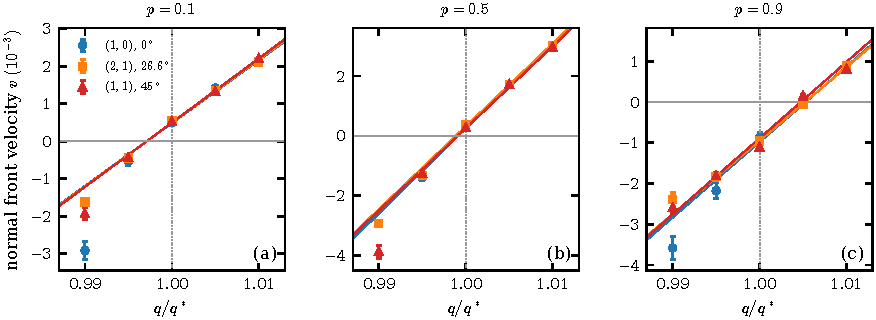
\includegraphics[width=\textwidth]{figs/fig_orient}
\caption{Normal velocity of a band of the active phase against the absorbing state, for normal
directions $(1,0)$, $(2,1)$, and $(1,1)$, at $p = 0.1$, $1/2$, and $0.9$; $L = 4096$, $T = 2\times10^5$,
eight seeds per point, velocity from the width of the band tracked along its normal for
$t\ge 10^4$. Lines: weighted fits through the four points at $q/\qs\ge 0.995$; at $0.99\,\qs$ the
interior of the band nucleates the absorbing phase within the fit window, which speeds its
retreat.}
\label{fig:orient}
\end{figure*}

\begin{figure*}
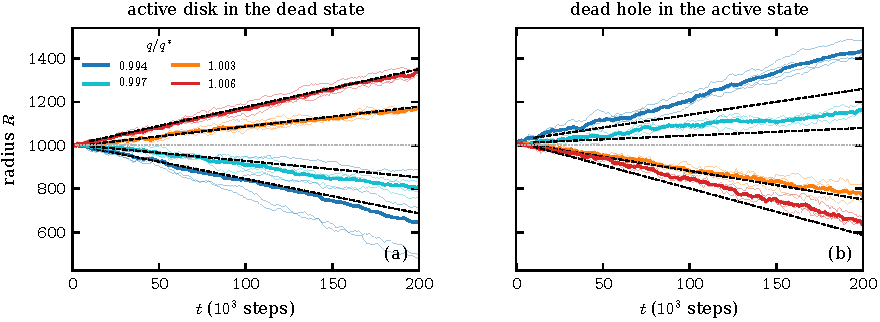
\includegraphics[width=\textwidth]{figs/fig_drop2}
\caption{Two-droplet test at $p = 1/2$ ($L = 4096$). Radius of (a) an active disk in the dead state
and (b) a dead hole in the active state, both of initial radius 1000, at $q/\qs = 0.994$, 0.997,
1.003, and 1.006 (thin lines: four seeds; thick lines: their mean); radii from the row profiles
(Appendix~\ref{app:numerics}). Dashed: $\ds R/\ds t = \pm v - D/R$ with $v = 0.28\,(q/\qs - 0.999)$,
the local slope and crossing of the $(1,0)$ band of Fig.~\ref{fig:orient}(b), and $D = 0.20$
(Fig.~\ref{fig:drop}).}
\label{fig:drop2}
\end{figure*}

\subsection{Bulk: the jump and the metastable active phase}
\label{sec:bulk}

Bulk runs from random initial conditions (Fig.~\ref{fig:bulk}) give the stationary interface
density of the active phase. Above $\qs$ it settles within $10^3$--$10^4$ steps and then stays
constant to the end of the runs ($t = 2\times10^5$--$10^6$), independently of $L$ from 256 to 4096
to within $10^{-4}$: $\rho = 0.3022$--$0.3023$ at $q = 1.008\,\qs$ and $0.3111$--$0.3113$ at $1.018\,\qs$
[Fig.~\ref{fig:bulk}(b)]. Even at $q = 0.998\,\qs$, within the uncertainty of $\qs$, the active phase
holds $\rho = 0.284$ for the full run ($10^6$ steps for $L\le 1024$, $3\times10^5$ and
$2\times10^5$ for $L = 2048$ and 4096) at every $L\ge 512$. There is no sign of $\rho\to 0$ as
$q\to\qs$: the density jumps from $0.28$ to zero. The magnetic susceptibility of the active phase,
$\chi_L = L^2\langle m^2\rangle$, grows toward the transition, from 63 at $1.098\,\qs$ to 430 at
$1.008\,\qs$ and $\approx 1300$ at $0.998\,\qs$, but at each $q$ it is independent of $L$ for
$L\ge 512$: the magnetization is correlated over a finite area, $\chi\approx 1300$ sites at the
transition, i.e., a correlation length $\xi\approx(\chi/2\pi)^{1/2}\approx 15$ for exponentially
decaying correlations. Measured directly from stored configurations at $1.009\,\qs$ ($L = 2048$,
$t\ge 10^5$), the two-point function of $m$ falls to $0.40$ at one lattice spacing and then decays
exponentially with $\xi = 15$--$18$ (fits over $4\le r\le 40$ and $10\le r\le 60$); at $1.1\,\qs$,
$\xi = 7$--$9$.

Below $\qs$ the active phase is metastable. At $q = 0.988\,\qs$ its density stays within 12\% of
the stationary value for $10^4$ steps and then collapses at an accelerating rate
[Fig.~\ref{fig:bulk}(a)], as droplets of the two absorbing phases nucleate and grow
[Fig.~\ref{fig:snap}(b)]; a critical decay would instead slow down with time. Where droplets of opposite type meet, a layer of the active phase
remains between them (Sec.~\ref{sec:wall}), so $\rho$ does not drop to zero at once but to a slowly
coarsening network of wetted walls. The half-life $\tau$ of the active state grows steeply as
$q\to\qs$: $\tau = 3.4\times10^3$, $8.0\times10^3$, $1.6\times10^4$, $2.6\times10^4$, and
$7.0\times10^4$ at $q/\qs = 0.899$, 0.949, 0.969, 0.979, and 0.988. For $L\ge 256$ it does not depend
on $L$ [Fig.~\ref{fig:bulk}(c)]: many droplets nucleate independently, and the decay is a local
process (the multi-droplet regime of Ref.~\cite{rikvold1994}). Smaller systems ($L\le 128$) decay
sooner, because their size is only a few correlation lengths of the active phase, so that
the whole lattice can reach an absorbing state through one fluctuation.

The size dependence above $\qs$ is the opposite, and it is the finite-size signature that
separates a stable phase from a long transient. At $q = 1.008\,\qs$ all 32 runs at $L = 64$
reached an absorbing state (median half-life $1.6\times10^4$), 25 of 32 runs at $L = 128$ decayed
(median $2\times10^5$), and none of the 16 runs at $L = 256$ or of the 8 runs each at $L = 512$
and 1024 decayed within $10^6$ steps; at $1.018\,\qs$ the counts are 32 of 32, 4 of 32, and 0 of
16; at $1.048\,\qs$, 31 of 32 at $L = 64$ and none at $L\ge 128$. Below $\qs$ the lifetime
saturates in $L$; above $\qs$ it grows faster than any power of $L$ and leaves the accessible
window between $L = 128$ and 256, as expected for a phase that can only be destroyed by a
fluctuation of the size of the system.
% Independent check (referee round 3, 2026-10-30; same code, q* = 0.04596, 24 seeds, T = 1e6):
% 1.008 q*: L = 64 24/24 decayed (median 3.2e4), L = 128 19/24 (2.2e5), L = 192 0/24, L = 256 0/24;
% 1.018 q*: 24/24 (3.6e4), 1/24, 0/24, 0/24. Per-run data: reports/tauL_check_2026-10-30.csv.

Over the accessible range, $\delta = 1-q/\qs$ from 0.1 to 0.012, the half-life grows roughly as
$\delta^{-1.4}$. In the multi-droplet regime $\tau\propto(Iv^2)^{-1/3}$, with $I$ the nucleation
rate per site and $v\propto\delta$ the growth velocity, so this corresponds to $I\propto\delta^{2.2}$.
Classical nucleation theory predicts instead $I\propto\exp(-B/\delta)$, which fits the five points
less well (rms deviation 13\% in $\tau$, against 5\% for the power law; $B\approx 0.06$). This is not
surprising: the critical radius at $\delta = 0.012$, $R_c\approx D/|v|\approx 70$
(Sec.~\ref{sec:drops}), is only about five correlation lengths of the active phase, so the
nucleation barrier is still small compared with the fluctuations that create absorbing patches,
and the asymptotic essential singularity lies at smaller $\delta$ than we can reach.

\begin{figure*}
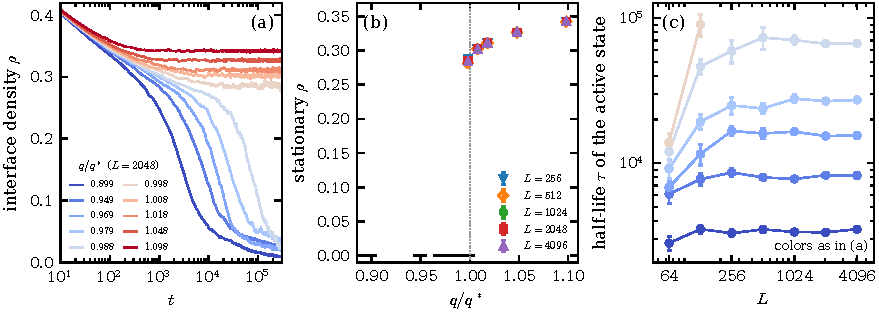
\includegraphics[width=\textwidth]{figs/fig_bulk05}
\caption{Bulk runs at $p = 1/2$ from random initial conditions ($\qs = 0.04596$). (a) Interface
density against time at $L = 2048$ for $q/\qs$ from 0.9 to 1.1 (one seed each). (b) Stationary density
against $q/\qs$ for $L = 256$--4096 (mean over $t\ge T/2$; 2--16 runs per point; bars at zero: the
active state decays). (c) Half-life of the active state below $\qs$ against $L$ (32 runs for $L\le
128$, 2--16 above; $T = 10^6$ for $L\le 1024$, $3\times10^5$ and $2\times10^5$ for $L = 2048$ and
4096).}
\label{fig:bulk}
\end{figure*}

\subsection{Critical droplets}
\label{sec:drops}

Above $\qs$ the active phase is stable, but a small region of it does not grow: an active droplet
in the absorbing state must exceed a critical size. We placed a disordered disk of radius $R$
(sites alive with probability $1/2$) in the dead state and ran 500--1000 independent replicas per
$(q, R)$ until the droplet died or reached the lattice edge (Fig.~\ref{fig:drop}). The survival
probability rises from 0 to 1 over a factor of about 3 in $R$, and the radius at which it reaches
$1/2$ grows as $q\to\qs$: $R_c = 2.6$, 4.8, 7.9, 12.5, 21, and 42 at $q/\qs = 2.0$, 1.40,
1.20, 1.10, 1.05, and 1.02. Plotted against the inverse planar-front velocity at the same $q$,
$R_c$ is linear [Fig.~\ref{fig:drop}(b)], $R_c\simeq D/v + \Delta R$ with $D = 0.20$ and an offset
$\Delta R = 1.6$ sites that accounts for the relaxation of the random initial disk; equivalently,
$R_c v = 0.21$--$0.26$ over a factor of 11 in $v$. This is the critical radius of the growth law $\ds R/\ds t = v - D/R$, in
which the curvature of the front slows a convex active region; it diverges as
$R_c\propto 1/(q-\qs)$ at the transition. A $2\times2$ block of live sites, the standard initial
condition of spreading experiments, is far below $R_c$: it survives with probability
$0.042\pm0.003$ at $q = 1.4\,\qs$ and $0.20\pm0.01$ at $2\,\qs$, and with probability $0.011$ at
$1.2\,\qs$ and $0.003$ at $1.1\,\qs$ (4000 replicas each), although the active phase is the stable
one there; the $R = 0.75$ disks of Fig.~\ref{fig:drop}(a), $2\times2$ blocks in which each site is
alive with probability $1/2$, survive with probability $0.014$ and $0.061$ at $1.4\,\qs$ and $2\,\qs$.
In a DP- or GV-type transition, by contrast, a single seed survives with finite probability
everywhere in the active phase, with no size threshold.

\begin{figure*}
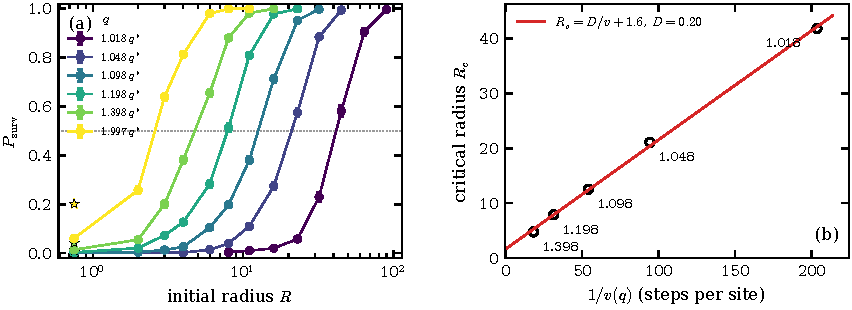
\includegraphics[width=\textwidth]{figs/fig_drop}
\caption{Critical droplets at $p = 1/2$. (a) Survival probability of a disordered disk of radius $R$
in the dead state, for $q/\qs$ from 1.02 to 2 (500--1000 replicas per point; at $R = 0.75$, a
$2\times2$ block with each site alive with probability $1/2$, 4000 replicas). Stars: the full
$2\times2$ block of live sites (4000 replicas). (b) Radius $R_c$ at
which $P_{\rm surv} = 1/2$ against the inverse velocity of a planar front at the same $q$; labels
give $q/\qs$. The line is $R_c = D/v + \Delta R$.}
\label{fig:drop}
\end{figure*}

\subsection{Wetting of the wall between the absorbing phases}
\label{sec:wall}

The two absorbing phases cannot convert into each other directly: a flat wall between all-alive
and all-dead regions (protocol v) moves only through the sites next to it. Below $\qs$ the wall
develops a layer of the active phase whose thickness is stationary and grows as $q\to\qs$
(Figs.~\ref{fig:snap}(c) and \ref{fig:wall}). We measure it by the number $I$ of interface sites
per unit length of wall. At $q = 0$ the bare wall carries $I_0 = 8.7$. Below $\qs$, $I$ reaches a
stationary value within $10^4$--$10^5$ steps and stays there to the end of the runs, $10^6$ steps
for $\delta\ge 0.02$ and $3\times10^6$ at $\delta\le 0.0065$ (successive $10^6$-step windows agree
to 2\%), and the excess $\Gamma = I - I_0$ is the same for $L_x = 256$, 1024, and 4096 and for
$L_y = 1024$, 2048, and 4096 to within 3\%: $\Gamma = 10.0$, 17.7, 27.5, 36.9, 45.7, 64.6, 87, and
109 at $\delta = 1-q/\qs = 0.20$, 0.10, 0.051, 0.031, 0.021, 0.011, 0.0065, and 0.0040. The layer
thickens without bound as $\delta\to 0$, and the interface-site fraction at its center rises toward
the bulk value [0.53 at $\delta = 0.0065$, against 0.74 in the bulk active phase;
Fig.~\ref{fig:wall}(b)], and $\Gamma\propto\delta^{-\psi}$ with a local exponent that settles at
$\psi = 0.5$--$0.55$ for $\delta\le 0.05$ and stays there down to $\delta = 0.0040$, where the layer
is 190 rows thick [Fig.~\ref{fig:wall}(c)]. The uncertainty of $\qs$ (0.1\%) moves the small-$\delta$
points, by a quarter of $\delta$ at the smallest, and we quote $\psi = 0.5\pm0.06$ over the window. A
fit $\Gamma = A\delta^{-1/3} + B$ reproduces the points to within 3\% but needs $B = -32$, larger
in magnitude than $\Gamma$ at $\delta = 0.05$. The wetted wall also wanders along $y$: in runs of
$2$--$3\times10^6$ steps at $\delta\le 0.02$ a few walls drifted far enough to consume one of the
absorbing slabs, most often in the $L_x = 4096$, $L_y = 1024$ box, where the excursions of the
layer edges reach the other wall; those runs enter $\Gamma$ only before the drift, and the smallest
$\delta$ were run at $L_y = 4096$. At $\qs$ itself the layer grows without bound, and above $\qs$
its edges become fronts moving at the planar-front velocity. Near the voter point the same wetting
occurs, with much thicker layers (Sec.~\ref{sec:voter}).

The wall between the two absorbing phases is therefore completely wetted by the active phase at
the transition: the three phases coexist at $\qs$, and the absorbing--absorbing interface splits
into two absorbing--active interfaces. An active layer on the wall between two absorbing phases
has been seen before, in the four-species alliance model, where the two alliances coarsen like
Ising domains separated by a boundary layer in which the four species keep invading each
other~\cite{szabo2007}; here the layer has a stationary thickness that diverges at the
transition, and we can measure it. In equilibrium the analogue is the complete wetting of the
interface between two ordered phases by the disordered phase at a first-order Potts
transition~\cite{selke1983,carlon1999}; there, for short-range forces in two dimensions, thermal
fluctuations of the two interfaces give the excess adsorption a divergence with exponent
$1/3$~\cite{lipowsky1983,fisher1984,carlon1999}. Out of equilibrium, complete wetting has been
studied for a single bounded Kardar--Parisi--Zhang
interface~\cite{hinrichsen1997wet,munoz1998,delossantos2003}, not for a layer confined by two
fluctuating active--absorbing fronts. The effective exponent $\psi\approx 1/2$ found here is
larger than $1/3$. The edges of the layer are as rough as a free front: from stored configurations
(Appendix~\ref{app:numerics}) the height-difference correlation of either edge grows as
$r^{2\zeta}$ with $\zeta = 0.50\pm0.02$ for $r\le 50$, at every $\delta$ and $L_x$, exactly as for
the fronts of a band at $\qs$ [Fig.~\ref{fig:rough}(a)], so a walks-and-walls argument with
$\zeta = 1/2$ would give $\psi = 1/3$ here as well. That argument, however, needs the edges to
collide with each other many times along the wall, i.e., $L_x$ much larger than the collision
length $\xi_\parallel\approx w^2/25$ (from $C(r)\approx 25\,r$), which is 400--1200 for layers of
thickness $w = 100$--$170$. In our boxes the roughness of an edge grows with $L_x$ up to the
thickness of the layer (rms $28$, 50, and 87 at $L_x = 256$, 1024, and 4096 for $\delta = 0.011$,
where $w\approx 100$) without any change of $\Gamma$, so the thickness is not yet controlled by
the entropic repulsion of the edges; its distribution along the wall is broad, with a standard
deviation of half the mean and an exponential tail [Fig.~\ref{fig:rough}(b)]. Whether $\psi$
crosses over to $1/3$ for thicker layers and longer walls, or is the exponent of a different
mechanism (a diffusive penetration depth $\propto|v|^{-1/2}$ of the activity generated at the
wall would give $1/2$), we cannot decide with these sizes. At a continuous transition there is no
third phase to wet the wall; at a GV point the layer would broaden as at the voter point,
$W\propto t^{1/2}$, without a stationary value.

\begin{figure*}
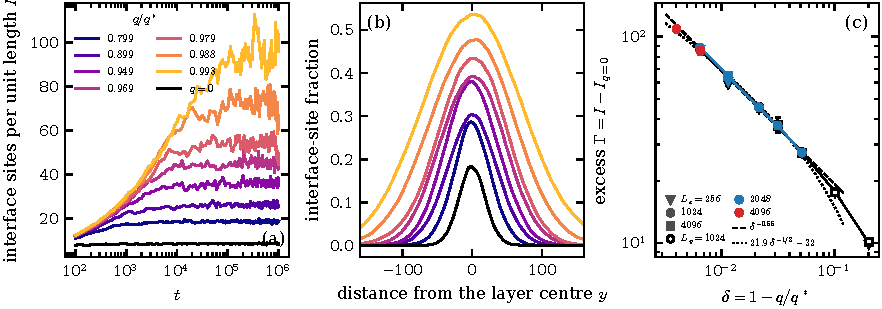
\includegraphics[width=\textwidth]{figs/fig_wall05}
\caption{Wetting of a flat wall between the two absorbing phases at $p = 1/2$ ($\qs = 0.04597$).
(a) Interface sites per unit wall length, $I$, against time at $L_x = L_y = 1024$ for $q/\qs$ from
0.80 to 0.993 and for $q = 0$ (mean of four seeds, $T = 10^6$). (b) Interface-site fraction across
the layer, each record centered on its interface-weighted mean row before averaging over
$t\ge 3.3\times10^5$. (c) Stationary excess $\Gamma = I - I_{q=0}$ against $\delta = 1-q/\qs$ for
$L_x = 256$, 1024, 4096 (triangles, circles, squares) and $L_y = 1024$ (open, $T = 10^6$,
$t\ge 3\times10^5$), 2048 and 4096 (filled, $T = 2$--$3\times10^6$, second half of each run); two to
four seeds per point. Lines: $\Gamma = A\delta^{-\psi}$ (dashed) and $A\delta^{-1/3} + B$ (dotted)
fitted to the $L_x = 1024$, $L_y\ge 2048$ points with $\delta\le 0.1$.}
\label{fig:wall}
\end{figure*}

\begin{figure*}
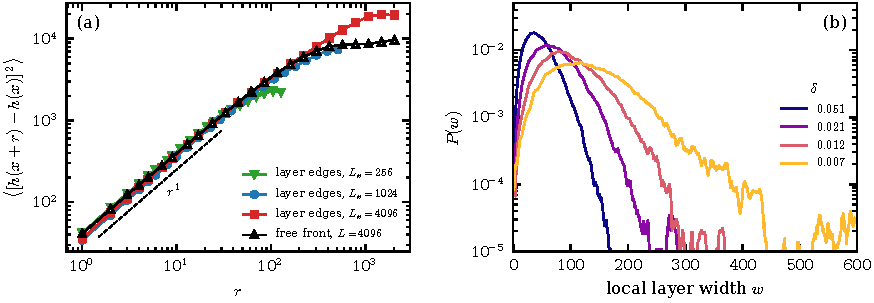
\includegraphics[width=\textwidth]{figs/fig_rough}
\caption{Edges of the wetting layer at $p = 1/2$, from configurations stored every $10^5$ steps for
$t\ge 10^5$ ($L_y = 2048$). (a) Height-difference correlation $\langle[h(x+r)-h(x)]^2\rangle$ of the
layer edges at $\delta = 0.011$ for $L_x = 256$, 1024, and 4096 (two to four seeds, both edges), and
of the two fronts of a band of the active phase at $\qs$ ($L = 4096$, eight seeds, $4\times10^4\le
t\le 2\times10^5$); the dashed line is $\propto r$, i.e., $\zeta = 1/2$. (b) Distribution of the
local thickness $w$ of the layer (per column) at $L_x = 1024$ for $\delta = 0.051$, 0.021, 0.011,
and 0.0065.}
\label{fig:rough}
\end{figure*}

%=====================================================================================
\section{The first-order line from Day \& Night to the voter point}
\label{sec:line}

\subsection{Phase diagram}
\label{sec:phase}

Figure~\ref{fig:phase} shows the transition line $\qs(p)$ from strip fronts at $\alpha = 1/2$,
together with the interface density of the active phase just above it. The line is nonmonotonic.
Starting from the D\&N limit, $\qs(0^+) = 0.0184$, it rises steeply (0.0207 already at $p = 0.01$)
to a maximum of $\approx 0.049$ near $p = 0.25$--$0.5$ and then falls linearly to zero at the voter
point, $\qs\approx 0.25\,\alpha(1-p)$ (Table~\ref{tab:line}). The initial rise reflects the voter
moves at $j = 4,5$, which D\&N forbids and which smooth interfaces. At every $p$ the front
velocity changes sign linearly at $\qs$ with a finite slope, the active phase behind a retreating
front keeps its interior density, and the bulk active density just above $\qs$ is finite,
$\rho_+ = 0.23$--$0.32$, with no trend toward zero along the line [Fig.~\ref{fig:phase}(b)]. We
find no tricritical point between the D\&N limit and $p = 0.995$.

\begin{table}
\caption{Transition line at $\alpha = 1/2$. $\qs$ from the zero of the strip-front velocity
($L_x = 2048$, $L_y = 4096$, $T = 10^5$, 2--4 seeds; $p\ge 0.99$: note $b$); $\qs\,\ds v/\ds q$ is
the dimensionless slope of $v(q)$ through $\qs$ over $\qs<q\le 1.065\,\qs$ (sites per step);
$\rho_+$ is the stationary bulk interface density at $q/\qs = x_+$, the lowest grid point above
$\qs$ ($L\ge 2048$, $T = 10^5$; $p\ge 0.98$: $T = 10^6$--$1.5\times10^6$); $c = \qs/[\alpha(1-p)]$.}
\label{tab:line}
\begin{ruledtabular}
\begin{tabular}{llllll}
$p$ & $\qs$ & $\qs\,\ds v/\ds q$ & $x_+$ & $\rho_+$ & $c$ \\
\hline
$0^{\,a}$ & 0.01837 & 0.08 & 1.007 & 0.227 & -- \\
0.01 & 0.02070 & 0.10 & 1.014 & 0.245 & 0.042 \\
0.02 & 0.02280 & 0.13 & 1.023 & 0.256 & 0.047 \\
0.05 & 0.02874 & 0.13 & 1.009 & 0.257 & 0.061 \\
0.1 & 0.03680 & 0.14 & 1.030 & 0.288 & 0.082 \\
0.25 & 0.04932 & 0.19 & 1.023 & 0.307 & 0.132 \\
0.5 & 0.04596 & 0.22 & 1.008 & 0.302 & 0.184 \\
0.75 & 0.0276 & 0.22 & 1.037 & 0.316 & 0.221 \\
0.9 & 0.01194 & 0.11 & 1.022 & 0.290 & 0.239 \\
0.95 & 0.00619 & 0.10 & 1.050 & 0.289 & 0.248 \\
0.98 & 0.00252 & 0.06 & 1.02 & 0.260 & 0.252 \\
0.99$^{\,b}$ & 0.00128 & 0.04 & 1.00 & 0.241 & 0.256 \\
0.995$^{\,b}$ & 0.00064 & 0.03 & 1.00 & 0.234 & 0.256 \\
\end{tabular}
\end{ruledtabular}
\begin{flushleft}\footnotesize
$^{a}$Limit $p\to 0^+$; at $p = 0$ itself the model has additional frozen configurations
(Appendix~\ref{app:frozen}).\\
$^{b}$Runs of $1.2\times10^6$ ($p = 0.99$) and $1.6\times10^6$ steps ($p = 0.995$), four times the
crossover time $t_\times$ of Sec.~\ref{sec:voter}, four seeds, velocities fitted for $t\ge t_\times$
from the outer envelope of the strip (Appendix~\ref{app:numerics}); from runs of $10^5$ steps the
crossing at $p = 0.995$ is 0.00062 (Sec.~\ref{sec:voter}).
\end{flushleft}
\end{table}

\begin{figure}
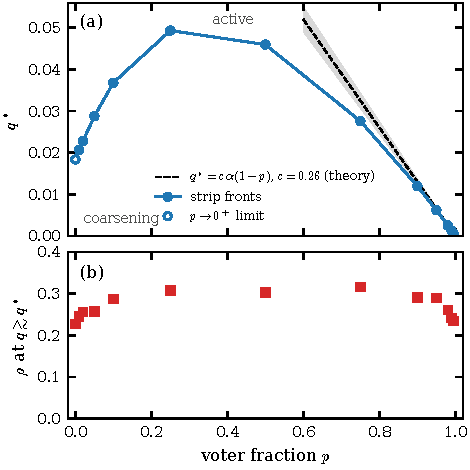
\includegraphics[width=\columnwidth]{figs/fig_phase}
\caption{(a) Transition line $\qs(p)$ at $\alpha = 1/2$ from strip fronts (Table~\ref{tab:line}). Open
circle: the limit $p\to 0^+$. Dashed: the voter-point theory $\qs = c\,\alpha(1-p)$ with $c = 0.26$, and
its uncertainty band. (b) Stationary interface density of the active phase at the lowest $q$ above
$\qs$ at which the bulk is stationary ($x_+$ in Table~\ref{tab:line}).}
\label{fig:phase}
\end{figure}

\subsection{Near the voter point}
\label{sec:voter}

As $p\to 1$ the transition approaches the voter point, where logarithmic corrections make every
diagnostic slow. The active density in the voter model itself decays as $1/\rho = 0.184\ln t +
2.13$ (our measurement at $L = 4096$ up to $t = 10^6$), so a density that looks stationary over a
finite window is not enough. We therefore checked four independent signatures at $p = 0.98$,
$0.99$, and $0.995$, with the noise strength measured by $\delta = q/\qs - 1$.

\textit{Bulk plateaus.} Runs to $t = 10^6$--$1.5\times10^6$ at $L = 2048$ (two to four seeds)
and $L = 4096$ hold a stationary plateau $\rho\approx 0.23$--$0.26$ down to within 2\% of the
threshold at $p = 0.98$ ($\delta = 0.02$) and to the threshold itself at $p = 0.99$ and $0.995$
($\delta\le 0.003$); the plateaus at the two sizes agree to within 0.003 ($0.01$ at $p = 0.995$,
$\delta = 0$). The strip crossing and the bulk threshold agree only once the strips are run past
the wall crossover time $t_\times$ found below ($\approx 3\times10^5$ and $4\times10^5$ at
$p = 0.99$ and $0.995$): from runs of $10^5$ steps the crossing at $p = 0.995$ is $q = 0.00062$,
where the bulk active phase decays within $1.5\times10^6$ steps at both sizes; strips run to
$1.6\times10^6$ steps retreat and dissolve there, and their velocity for $t\ge t_\times$ crosses
zero at $\qs = 0.00064$ (four seeds, $\pm0.000005$), 3\% higher, where the bulk is stationary to
$1.5\times10^6$ steps and decays 0.6\% lower. The same rerun at $p = 0.99$ ($1.2\times10^6$
steps) confirms $\qs = 0.00128$; Table~\ref{tab:line} lists the late-time values. Just below
the threshold the active state is metastable for $10^5$--$10^6$ steps and then collapses. The
plateau decreases slowly toward the threshold: at $p = 0.99$, $1/\rho$ grows from 3.60 at
$\delta = 0.19$ to 4.11 at $\delta = 0$, roughly linearly in $\ln(1/\delta)$ for $\delta\ge 0.01$.
Over this range this is equally consistent with a finite jump and with a jump vanishing
logarithmically, which is why the next three tests are needed.

\textit{No Ising ordering in the active phase.} A split into an Ising and a DP transition would
leave an ordered active window, with $\chi_L = L^2\langle m^2\rangle\sim L^{7/4}$ at the Ising
point. At $p = 0.98$ and $0.99$, for $\delta$ from $0$ to $0.2$, $\chi_L$ saturates for $L\gtrsim
1024$--$2048$ (Fig.~\ref{fig:voter}(a)): its ratio between $L = 4096$ and 2048 is 0.76--1.14,
against 3.4 for Ising, the Binder cumulant stays near zero, and the relaxation time of $m$ is
independent of $L$. The correlated area of the magnetization, $\chi\approx 10^4$--$6\times10^4$
sites at $1.00$--$1.02\,\qs$ ($\xi\approx 40$--$100$), grows toward $p = 1$ but not with $L$. At
$p = 0.995$ the
size dependence is weaker than Ising but not flat ($\chi_{4096}/\chi_{2048} = 1.8\pm0.6$).

\textit{Seeds die faster than voter seeds.} A $2\times2$ block of live sites in the dead state
spreads, in the voter model, with survival probability $P_s(t)\simeq A\ln t/t$~\cite{bramson1980},
i.e., a local exponent $\delta_{\rm eff} = -\ds\ln P_s/\ds\ln t$ approaching 1 from below. At a GV
point the same holds, and at a DP point $\delta_{\rm eff}\to 0.451$. Figure~\ref{fig:voter}(b)
shows $t\,P_s(t)$, which grows as $\ln t$ for the voter model. At points where the bulk active
phase is stationary, it instead decreases: $\delta_{\rm eff}$ exceeds 1 and keeps rising, from 1.16 to 1.54 between $t = 3\times10^3$ and $3\times10^4$ at $(p,\delta) =
(0.98, 0.02)$, and from 0.97 to 1.13 at $(0.995, 0.017)$. Seeds die faster than voter seeds even
though the bulk active phase is stable, and their decay accelerates: a seed has to outgrow a
critical droplet before it can spread. At $(0.99, 0.01)$ the decay is still accelerating at
$t = 10^6$ ($\delta_{\rm eff} = 2.1$, $P_s(10^6) = 1.0\times10^{-6}$ against $1.9\times10^{-5}$ on the
voter curve), and at $(0.995, -0.012)$, just below the threshold, none of
$3\times10^6$ seeds survives to $10^6$. Further above threshold the seeds overshoot and then level off: at $(0.99, 0.04)$, running to
$t = 10^6$ on $L = 8192$ with $7.5\times10^5$ replicas, $P_s(10^6)/P_s(10^5) = 0.46\pm0.06$,
against 0.12 for the voter model, and $P_\infty>0$. The onset of $P_\infty$ is steep: at
$p = 0.98$, $P_\infty\approx 1.7\times10^{-4}$ at $\delta = 0.07$, $6\times10^{-5}$ at $0.05$, and no
plateau by $5\times10^5$ steps at $0.03$.

\textit{Walls are wetted below the threshold.} A flat wall between the two absorbing phases
(protocol v) roughens like a voter interface at first, $W\propto t^{1/2}$, independent of $q$. After
a crossover time $t_\times$, $q$ takes over (Fig.~\ref{fig:voter}(c)). Below $\qs$ ($\delta =
-0.02$ at $p\le 0.98$, $-0.03$ at $0.99$, $-0.05$ at $0.995$) the wall turns into a slab of the
active phase of stationary width, $W(10^6)\approx 200$,
450, 670, and 820 for $p = 0.9$, 0.98, 0.99, 0.995, whose interior has an interface-site
fraction of 0.46--0.51, as in the bulk active phase at $\qs$ (0.47--0.58); the pure voter wall
keeps widening. Above
$\qs$ the slab edges move outward at the strip-front velocities. The crossover time grows as
$t_\times\propto(1-p)^{-1.3}$, from $\approx 10^4$ at $p = 0.9$ to $\approx 4\times10^5$ at $p =
0.995$; it is the time the perturbation of the voter model needs to act, and it is why the
order of the transition cannot be settled numerically for $p>0.995$.

Together, these results place a first-order transition at every $p\le 0.995$ we studied: a GV
point would need a $q_c$ at which the bulk is active, seeds decay no faster than voter seeds, and
walls broaden diffusively, and none of the points between $\qs$ and $1.2\,\qs$ at
$p = 0.98$--$0.995$ behaves like that.

\begin{figure*}
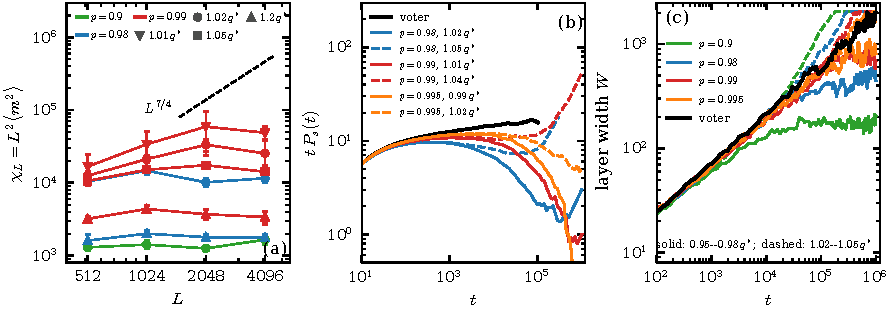
\includegraphics[width=\textwidth]{figs/fig_voter}
\caption{Near the voter point. (a) Magnetic susceptibility $\chi_L = L^2\langle m^2\rangle$ of the
active phase against system size, at $q/\qs = 1.0$--$1.2$ (markers; the legend gives $q/\qs$ to
within 1\%) for $p = 0.9$, 0.98, 0.99 (colors); 4--8 runs to $t = 10^6$ per point,
$t\ge 2\times10^5$. The dashed line is the Ising law $L^{7/4}$. (b) Survival of a $2\times2$ seed in
the dead state, $t\,P_s(t)$, which grows as $\ln t$ for the voter model (black, $L = 2048$), decays
when the seed must outgrow a critical droplet, and grows linearly once $P_\infty>0$; $3\times10^6$
replicas per point (fewer at the upper $q$ of each $p$) on $L = 8192$. (c) Width $W$ of the active
layer on a flat wall between the two absorbing phases, $L_x = 1024$, $L_y = 4096$, two seeds, below
$\qs$ (solid: $0.98\,\qs$ at $p\le 0.98$, $0.97\,\qs$ at $0.99$, $0.95\,\qs$ at $0.995$) and above it
(dashed: $1.05$, $1.04$, and $1.02\,\qs$); black: the voter model ($p = 1$, $q = 0$).}
\label{fig:voter}
\end{figure*}

\subsection{Synchronicity and asynchronous updating}
\label{sec:async}

The D\&N weight $\alpha$ sets the scale of $\qs$. Near the voter point the threshold is exactly
proportional to $\alpha$: strip fronts at $\alpha = 1/4$, $1/2$, and 1 for $p = 0.98$ and 0.99 give
$\qs\propto\alpha^{\beta}$ with $\beta = 1.00\pm0.02$ and $c = \qs/[\alpha(1-p)] = 0.248$--$0.258$
(Table~\ref{tab:alpha}), as the theory of Sec.~\ref{sec:theory} predicts. In the D\&N limit the
jump persists at every $\alpha$ from $1/8$ to 1, with no sign of a tricritical point.

Synchronous updating is a natural suspect for any unusual behavior of a cellular automaton, and
the GV and voter classifications refer to continuous-time dynamics. We therefore made the
dynamics lazy: each site is updated with probability $r$ per step (the flip table is multiplied
by $r$), so $r\to 0$ is continuous time and $rt$ is the physical time. At $p = 0.98$ the front
velocity still changes sign linearly, now at $\qs(r)/\qs(1) = 0.864\pm0.010$, $0.858\pm0.016$,
and $0.870\pm0.012$ for $r = 1/2$, $1/4$, and $1/8$; the shift saturates by $r = 1/2$. At
$p = 0.99$, $r = 1/4$, fronts just above $\qs(r)$ retreat for $\sim 10^5$ physical time units
before advancing, and the late-time crossing, $0.85$--$0.88$, agrees with $p = 0.98$. At the
representative point $p = 1/2$ the shift is the same, $\qs(1/4)/\qs(1) = 0.867$ (three seeds), and
the bulk active phase at $1.014\,\qs(1/4)$ holds a stationary $\rho = 0.211$ up to physical time
$10^5$, while at $0.99\,\qs(1/4)$ it decays slowly. All the other signatures reappear at the
shifted threshold: bulk plateaus that
stay flat over a factor 40 in time at only $\approx 8\%$ above $\qs(r)$, seeds with $\delta_{\rm
eff}>1$ and rising at and below $\qs(r)$ and $P_s$ leveling off above it, and walls that become
stationary active slabs below $\qs(r)$ while the lazy-voter wall keeps widening. The first-order
transition is not an artifact of synchronous updating.

\begin{table}
\caption{Synchronicity and asynchrony near the voter point. Top: $\qs\propto\alpha$ (strip
fronts, four seeds; errors are seed bootstrap, systematic $\approx\pm2\%$). Bottom: lazy updating
with probability $r$ per step at $p = 0.98$ and $1/2$; $c(r)$ from simulation and, near the voter
point, from the theory of Sec.~\ref{sec:theory}.}
\label{tab:alpha}
\begin{ruledtabular}
\begin{tabular}{lllll}
$p$ & $\alpha$ & $\qs$ & $c$ (sim.) & $c$ (theory) \\
\hline
0.98 & 0.25 & 0.001274(9) & 0.255 & \\
0.98 & 0.5 & 0.002515(19) & 0.252 & \\
0.98 & 1 & 0.005074(30) & 0.254 & 0.260(15) \\
0.99 & 0.25 & 0.000621(18) & 0.248 & \\
0.99 & 0.5 & 0.001292(7) & 0.258 & \\
0.99 & 1 & 0.002553(9) & 0.255 & \\
\hline
$p$ & $r$ & $\qs(r)/\qs(1)$ & $c(r)$ (sim.) & $c(r)$ (theory) \\
\hline
0.98 & 1/2 & 0.864(10) & 0.218 & 0.223(3) \\
0.98 & 1/4 & 0.858(16) & 0.216 & 0.208(4) \\
0.98 & 1/8 & 0.870(12) & 0.219 & 0.201(4) \\
0.5 & 1/4 & 0.867(7) & 0.159 & -- \\
\end{tabular}
\end{ruledtabular}
\end{table}

%=====================================================================================
\section{Theory near the voter point}
\label{sec:theory}

Near $p = 1$ the model is a small perturbation of the voter model, and the transition line can be
computed. Write Eq.~\eqref{eq:rule} as
\begin{equation}
w(j) = \frac{j}{8} + \varepsilon\, g(j),\qquad
g(j) = \alpha R(j) - \frac{j}{8} + \kappa\,\delta_{j,2},
\label{eq:pert}
\end{equation}
with $\varepsilon = 1-p$ and $\kappa = q/(1-p)$. In the theory of voter-model perturbations of
Cox, Durrett, and Perkins~\cite{cox2013}, which is formulated for $d\ge3$, on time scales of
order $1/\varepsilon$ the local density $u$ of live sites
evolves by the diffusion inherited from the voter model plus a reaction term $\varepsilon f(u)$,
\begin{equation}
f(u) = \big\langle (1-\sigma_0)\,g(j_0) - \sigma_0\, g(j_0)\big\rangle_u ,
\label{eq:f}
\end{equation}
where the average is over the voter model's local state at density $u$: a dead origin turns live
at rate $g(j_0)$ and a live one dies at rate $g(j_0)$. By duality, the states of the origin and
of its eight neighbors are those of the coalescing random walks started from these nine sites
and run backward for a time $T$; sites whose walks have coalesced share a state, and the
distinct lineages are independently live with probability $u$. For the synchronous Moore voter
model the walks are synchronous random walks on the Moore neighborhood, which we simulate
directly ($10^6$ samples of the nine walks per $T$).

The structure of $f$ follows from three exact properties. A $g$ linear in $j$ gives $f\equiv 0$,
so the voter part and the $-j/8$ term drop out. Patterns with one or two lineage classes cancel
by the up--down symmetry. A pattern with three classes, in which the two classes not containing
the origin hold $n_1$ and $n_2$ neighbors, contributes
\begin{equation}
u(1-u)(1-2u)\,\big[g(n_1)+g(n_2)-g(n_1+n_2)\big],
\label{eq:three}
\end{equation}
four-class patterns contribute to the same cubic, and patterns with five or more classes
contribute polynomials of degree five and higher. Hence $f = \alpha f_R +
\kappa f_2$ exactly, every threshold is of the form $\kappa^* = \alpha\times$(a pure number),
and the transition line is
\begin{equation}
\qs = c\,\alpha\,(1-p)\qquad (p\to 1).
\label{eq:line}
\end{equation}
Two thresholds follow from $f$: $\kappa_a$, where $f'(0) = 0$ and the absorbing state loses linear
stability, and $\kappa_{\rm front}$, where $\int_0^{1/2} f\,\ds u = 0$ and a front between the
absorbing state and the active state $u = 1/2$ is stationary, the sign of the front speed being
that of the integral~\cite{durrett1994b,durrett2009}. Between them both $u = 0$ and
$u = 1/2$ are stable and the reaction--diffusion equation has a first-order transition at
$\kappa_{\rm front}$; this is the two-dimensional counterpart of Case~4A of
Ref.~\cite{cox2013}, where coexistence holds although $f'(0)<0$.

In two dimensions all lineages eventually coalesce, the reaction function of
Ref.~\cite{cox2013} is not defined~\cite{cox2025}, and we use a closure: the pattern weights are
evaluated for walks run for a finite time $T$, which plays the role of $1/\varepsilon$ up to an
undetermined factor of order one, and they decay as powers of $1/\ln T$. The closure assumes that
the local statistics on the scale $T$ are those of the voter model; it is a heuristic, not a
limit theorem, and we know of no precedent for it in $d = 2$. Three-class patterns give the
cubic~\eqref{eq:three}, whose sign on $0<u<1/2$ is fixed, so they cannot make both $u = 0$ and
$u = 1/2$ stable; four-class patterns give the same cubic, with coefficient
$g(n_1)+g(n_2)+g(n_3)-g(n_1+n_2+n_3)$; bistability comes only from patterns with five or more
classes, which contribute polynomials of degree five and higher and whose relative weight falls
as $T$ grows: they make up 43\% of the patterns with at least three classes at $T = 64$, 15\% at
$T = 1024$, and 3.6\% at $T = 65536$. Accordingly the two thresholds close in on each other from opposite sides
(Fig.~\ref{fig:theory}): $\kappa_a/\alpha = 0.355$, $0.289$, $0.265$ and $\kappa_{\rm front}/\alpha
= 0.231$, $0.249$, $0.255$ at $T = 64$, 1024, 65536, with bootstrap errors $\approx 0.002$.
Extrapolations in $1/\ln T$ are not reliable, and we quote the bracket,
\begin{equation}
c = 0.26\pm0.015 .
\label{eq:c}
\end{equation}
The simulations give $c = 0.239$, 0.248, 0.252, 0.256, and 0.256 at $p = 0.9$, 0.95, 0.98, 0.99,
and 0.995 (Table~\ref{tab:line}) and $c = 0.248$--$0.258$ with $\qs\propto\alpha$ at $p = 0.98$
and 0.99 (Table~\ref{tab:alpha}), between 1.5\% and 8\% below the center of the bracket. There is
no fitted parameter, but the matching scale is not fixed by the theory: at $T = 1/(1-p)$ the
closure gives $\kappa_{\rm front}/\alpha = 0.20$--$0.24$ for $p = 0.9$--$0.995$, 6--16\% below the
simulations, and the bracket~\eqref{eq:c} is its $T\to\infty$ limit. What the theory predicts
exactly is the structure $\qs\propto\alpha(1-p)$; the amplitude it gives to within about ten
percent.

\begin{figure}
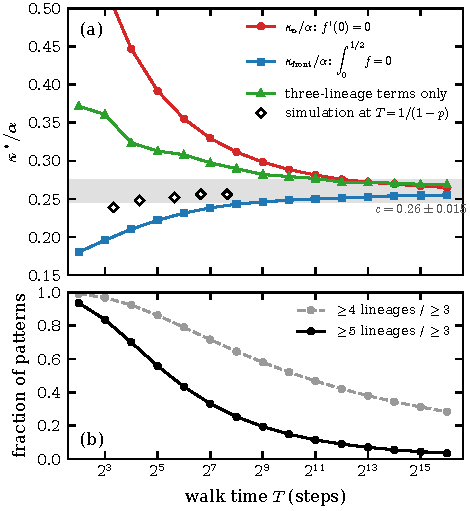
\includegraphics[width=\columnwidth]{figs/fig_theory}
\caption{Voter-point perturbation theory. (a) Thresholds $\kappa^*/\alpha$, with $\kappa = q/(1-p)$,
against the duration $T$ of the coalescing walks: loss of stability of the absorbing state
($\kappa_a$), stationary front ($\kappa_{\rm front}$), and the threshold from three-lineage
patterns alone; bootstrap errors are smaller than the symbols. Diamonds: simulated
$c = \qs/[\alpha(1-p)]$ for $p = 0.9$--$0.995$, placed at $T = 1/(1-p)$. Gray band: $c = 0.26\pm0.015$.
(b) Fraction of patterns with five or more lineages among those with at least three (black);
these patterns alone can make the reaction term bistable. Gray: four or more lineages.}
\label{fig:theory}
\end{figure}

The same calculation with lazy walks, each lineage moving with probability $r$ per step, is the
dual of the lazy dynamics of Sec.~\ref{sec:async}. It predicts $c(r) = 0.223\pm0.003$,
$0.208\pm0.004$, and $0.201\pm0.004$ at $r = 1/2$, $1/4$, and $1/8$, against $0.218$, $0.216$,
and $0.219$ in the simulations: the theory gets the sign of the shift and its size between $r = 1$
and $r = 1/2$, but continues to decrease below $r = 1/2$ while the simulations do not. The
residual 4--8\% at small $r$ is a discrepancy that the leading-order closure does not resolve.

The theory also explains how the first-order line ends. The coexistence window
$[\kappa_{\rm front},\kappa_a]$ exists only through the five-class terms, so at small
$\varepsilon$ it closes as a power of $1/\ln(1/\varepsilon)$. The transition is first order at
every $p\le 0.995$ we studied, and the closure suggests that it remains so at every fixed $p<1$,
only logarithmically so as $p\to 1$, with the voter point as a marginal endpoint of the
first-order line; we state this as a conjecture. The same logarithmic pinching appears in the rigorous theory
of the two-dimensional Lotka--Volterra model, whose coexistence region near the voter point is a
thorn of width $\propto 1/[\ln(1/\varepsilon)]^2$~\cite{cox2010}. It is consistent with the
slow weakening of the signatures in Sec.~\ref{sec:voter}: the shrinking front slope, the
decreasing plateau, and the crossover time $t_\times$ that grows as $p\to 1$.

%=====================================================================================
\section{Discussion}
\label{sec:discussion}

We have shown that a two-dimensional lattice model with exactly two $\mathbb{Z}_2$-symmetric
absorbing states can have a discontinuous transition into them, with all the hallmarks of phase
coexistence, and that this transition persists along a line running from the D\&N limit to
within half a percent of the voter point. The result contradicts the expectation that every such
transition in two dimensions is either of GV type or an Ising--DP
split~\cite{dornic2001,alhammal2005,castellano2009}.

What is new is the setting, not the phenomenology. Stationary fronts that reverse linearly,
Ising-like coarsening of the two absorbing phases, and an active layer between them were all
seen in the four-species alliance models~\cite{szabo2004,szabo2007,guisoni2013}, and a jump of
the order parameter into one of three symmetric absorbing states in a Potts-like
model~\cite{lipowski2002,azizi2018}. In those models the absorbing phases are sets of
configurations with internal dynamics, or there are more than two of them, and the generalized
voter theory does not apply. Here the absorbing states are two configurations, the setting of
the Langevin equation of Ref.~\cite{alhammal2005}; the transition was expected to be continuous;
and Molofsky \emph{et al.}~\cite{molofsky1999} had looked for the bistable regime in the simplest
synchronous nonlinear voter automaton and found none. The new results are the first-order
transition itself, established by the full set of coexistence tests; the finite-size behavior of
the lifetime, which saturates below $\qs$ and explodes above it; the wetting layer with a
stationary thickness that diverges at $\qs$; the first-order line that reaches the neighborhood
of the voter point; and the lineage calculation that gives the position of a rule's transition
line near it and the width of the band in which its absorbing states are metastable, which a
direct simulation of the rule of Molofsky \emph{et al.} confirms and which explains why their
search found none (Appendix~\ref{app:molofsky}). The same simulation shows that the fully
first-order transition is not generic in the class: their rule has the metastable absorbing
state but no metastable active phase.

Why is the bistability not washed out? The washout argument~\cite{castellano2009} pictures the
active phase as the symmetric point $\phi = 0$ of a single field and lets noise carry the system
over a mean-field barrier into an absorbing state. Here the active phase is a phase in its own
right, with a finite correlation length and its own interface density, and in two dimensions the
competition between two locally stable phases is decided by the motion of the fronts between them.
A fluctuation that converts a region of the active phase into an absorbing state must create a
domain larger than a critical droplet, whose cost grows as the transition is approached; below
the transition such domains nucleate and grow, above it they shrink. This is ordinary
two-dimensional first-order behavior, made possible by the surface-tension-like
curvature term in the droplet dynamics, which one-dimensional systems lack~\cite{hinrichsen2000fo}.
In the language of voter-model perturbations, the active phase wins against linearly stable
absorbing states by invasion, the scenario proven in $d\ge3$ as Case~4A of Ref.~\cite{cox2013}.
In the five-cell automaton of Molofsky \emph{et al.} seeds of one or two sites nucleated the
active phase at every parameter they tried~\cite{molofsky1999}. The closure of
Sec.~\ref{sec:theory}, applied to their rule (Appendix~\ref{app:molofsky}), locates the
difference not in a sign but in a weight: five lineages started on a plus stay distinct ten to
forty times more rarely than nine started on a $3\times3$ block, so the band in which their
absorbing state is metastable is an order of magnitude narrower than ours and lies within
$2\times10^{-3}$ of a line through the voter point, where their search could not resolve it.
Simulated there, their rule shows the band, with the critical nucleus $R_c = D/v$ of
Sec.~\ref{sec:drops}, and the stationary front. It does not show a metastable active phase:
that phase coarsens away as soon as the front stops, whereas for D\&N it decays by nucleation,
after a plateau and with an $L$-independent lifetime, down to $0.9\,\qs$ (Sec.~\ref{sec:bulk}).
The terms responsible for the band are those that the first-derivative closure of
Ref.~\cite{vazquez2008} discards; what sets the extent of the active-state branch, which the
closure overstates for the five-cell rule, we do not know.

The previous evidence for washout came from the immediate neighborhood of the voter point, from
rules monotone or nearly linear in the number of disagreeing neighbors, and from strong noise.
Our theory shows why a first-order line can be invisible there: the coexistence window closes
logarithmically at the voter point. A stable active phase without noise is not new in itself---it
occurs in threshold voter models~\cite{liggett1994} and in other two-dimensional nonlinear voter
models~\cite{molofsky1999,lambiotte2007,schweitzer2009}---and what is new here is that the
transition into it is discontinuous. Monotonicity itself is not decisive---our model is monotone
for $p\ge 0.8$ and first order there too. What matters near the voter point is the
contribution of five or more coalescing lineages to the reaction term, which the rule's
nonlinearity in $j$ controls: its weight sets the width of the bistable window, and its sign
decides whether a given one-parameter family, such as $\kappa$ at fixed $\alpha$ here, crosses
it. The same calculation applies to any rule of the form~\eqref{eq:pert} and predicts, for each,
where its bistable window lies and how wide it is, which makes the classification testable rule
by rule. For the five-cell rule of Molofsky \emph{et al.} it predicts a window in the direction
of small $p_1$ and large $p_2$, in which they searched, around a line through the voter point of
slope $\ds p_2/\ds p_1\approx -3.5$ that coincides with their empirical boundary, but only
$4^\circ$ wide at $T = 16$ and $0.5^\circ$ at $T = 1024$. Planar fronts and droplets for their
rule (Appendix~\ref{app:molofsky}) find the line within $0.3^\circ$ and the absorbing-state
branch of the window with about the predicted width, and bound the active-state branch to less
than a thirtieth of its predicted width at $T = 16$ and a third of it at $T = 1024$: the closure
is quantitative for the line and for the metastability of the absorbing state, and it overstates
the stability of the active phase beyond the front reversal at every $T$, at least for a
five-cell neighborhood.

Several questions remain open. (i) The endpoint at the voter point: neither a renormalization
group treatment of the bistable term at the two-dimensional voter fixed point nor a rigorous
two-dimensional result exists~\cite{canet2005,cox2025}. (ii) Absorbing-state-breaking noise: a
small symmetric flip probability at $j = 0$ turns the two absorbing phases into ordered phases,
and the first-order line must then end, as the first-order line of the Ziff--Gulari--Barshad
model ends at a critical point once desorption is added~\cite{ziff1986,tome1993}, and as the
first-order lines of the alliance model end at directed-percolation critical points or meet at a
triple point~\cite{guisoni2013}; where and how it ends here is unknown. (iii) Quenched disorder,
which rounds first-order absorbing transitions in two dimensions when it locally favors one
phase~\cite{villamartin2014}; random fields are known to leave the transition between the two
absorbing states of a generalized contact process intact in two dimensions~\cite{barghathi2016},
and random fields and random bonds act differently on the two absorbing phases here. (iv) The
weak-noise, strongly bistable corner of the Langevin equation of Ref.~\cite{alhammal2005} (see
also Ref.~\cite{russell2011}), which has never been integrated in two dimensions and would tell
whether the continuum theory itself admits the transition found here. (v) A theory of the
wetting layer between the two absorbing phases (Sec.~\ref{sec:flagship}), a nonequilibrium
analogue of the complete wetting of the interface between two ordered phases at a first-order
Potts transition~\cite{selke1983,carlon1999} and of the boundary layer between
alliances~\cite{szabo2007}; the nonequilibrium wetting of a single bounded
interface~\cite{hinrichsen1997wet,delossantos2003} is the natural starting point.

\begin{acknowledgments}
\pending{Acknowledgments.} Simulations were run on the Torch cluster at New York University.
\end{acknowledgments}

\section*{Data availability}
The simulator (Appendix~\ref{app:numerics}), the campaign scripts, and the raw run outputs that
support this study are available from the authors upon request. \pending{Add a repository DOI if
deposited.}

%=====================================================================================
\appendix

\section{Frozen configurations at $p = 0$}
\label{app:frozen}

At $p = 0$ the flip table is $w(j) = \alpha R(j) + q\,\delta_{j,2}$, so every configuration in
which all sites have $j\in\{0,1,4,5\}$ is frozen. We counted these configurations with a transfer
matrix on strips of width $W = 7$ and $8$ with periodic boundaries: their number grows as
$e^{sN}$ with $s\approx 0.32$ per site, against $\ln 2 = 0.69$ for all configurations. As a check,
on the $3\times3$ torus, where every site neighbors every other, the count is
$254 = 1 + \binom94 + \binom95 + 1$. The simplest examples are the two checkerboards and the
diagonal stripes of width two, in which every site has $j = 4$.

These configurations are dynamically irrelevant for $q>0$. Random initial conditions at $L = 256$
run to $t = 10^6$ at $q = 0.005$--$0.018$ (all below $\qs$) end in one of the two uniform states.
In the active phase ($q = 0.03$--$1$) the frequency of locally checkerboard or stripe-like
$3\times3$ blocks stays at the level expected by chance. A prepared half-lattice of either pattern
next to an active or a dead half is eroded completely within $10^4$ steps at every $q$ tested,
including $q = 0$, and a single flipped site destroys a perfect $256\times256$ pattern within
$\approx 10^3$ steps (in 11 of 12 runs). Only at $q = 0$, where $j = 2$ sites are also frozen, does
the dynamics stop with a small density ($\approx 1\%$) of frozen debris.

Removing the frozen configurations directly by a flip probability $\epsilon$ at
$j\in\{1,4,5\}$ preserves the linear reversal of the front velocity: at $\epsilon = 0.003$ the
velocity is $-0.0041$, $-0.0002$, $+0.0024$, $+0.0053$ at $q/\qs(0) = 0.88$, 0.92, 0.96, 1.00, so
$\qs(\epsilon)\approx 0.92\,\qs(0)$, and at $\epsilon = 0.01$, $\qs\approx 0.8\,\qs(0)$, with
an interior interface fraction 0.44--0.6 behind the front. The $p = 0$ results are therefore the
$\epsilon\to 0^+$ limit of a model with exactly two absorbing states.

\section{Pair approximation}
\label{app:pa}

We closed the dynamics at the level of nearest-neighbor pairs on a Bethe lattice with $z = 8$:
given a site's state, its neighbors are independent and disagree with it with probability
$\theta_s = \rho/(2x_s)$, where $\rho$ is the fraction of disagreeing bonds and $x_s$ the fraction
of sites in state $s$. Both the continuous-time version and the synchronous map were analyzed.
In the voter limit the closure conserves $m$ and gives $\rho^* = (z-2)(1-m^2)/[2(z-1)]$. For every
$p<1$ a dilute minority in an absorbing state decays at rate
$(1-p)\alpha P_R(\theta) + qP_2(\theta)$, so the absorbing states are linearly stable, and the
symmetric active fixed point ($\rho^*\approx 0.43$--$0.50$) is stable at every $q\ge 0$, $p<1$,
and $\alpha$ checked. The approximation is bistable everywhere and has no transition of its own; a
front criterion based on it gets $\qs\propto(1-p)$ near the voter point but with an amplitude off
by a factor of two, and fails qualitatively for $p\lesssim 0.5$. This is why we rely on the
perturbation theory of Sec.~\ref{sec:theory}.

\section{A second rule: noise on the forbidden flips of D\&N}
\label{app:eta}

To check that the discontinuity does not depend on the voter admixture, we studied the rule
\begin{equation}
w(j) = \alpha R(j) + \eta\,[\,j\in\{1,2,4,5\}\,],
\label{eq:eta}
\end{equation}
in which every flip that D\&N forbids, except at $j = 0$, happens with a small probability $\eta$.
By the lemma of Sec.~\ref{sec:lemma} it has exactly two absorbing states. At $\alpha = 1/2$, strip
fronts ($L_x = 2048$, $L_y = 4096$, $T = 10^5$, three seeds) retreat at $v = -0.0022\pm0.0010$ for
$\eta = 0.01275$ and advance at $v = +0.0020\pm0.0001$ and $+0.0054\pm0.0001$ for $\eta = 0.013125$
and $0.01375$, so $\eta^*\approx 0.0130$ (linear interpolation: $0.01295$). Bulk runs at $L = 1024$ and 2048 (two seeds each,
$T = 2\times10^5$) hold a stationary interface density $\rho = 0.252$ at $\eta = 0.013125$ ($\approx
1.01\,\eta^*$) and $\rho = 0.275$ at $0.01375$, at both sizes. Below $\eta^*$ the active phase is
metastable: at $\eta = 0.01275$ it decays slowly (from $\rho = 0.236$ at $t = 10^4$ to $0.17$ at
$2\times10^5$), and at $\eta = 0.0125$, $0.01225$, $0.011875$, and $0.01125$ its half-life is
$(5.4$--$6.4)\times10^4$, $(2.6$--$3.2)\times10^4$, $(1.3$--$1.6)\times10^4$, and $(0.8$--$0.9)
\times10^4$, the same at both sizes. The transition is discontinuous, with a jump $\rho\approx 0.25$,
as in the voter-admixed family (Fig.~\ref{fig:eta}).

\begin{figure}
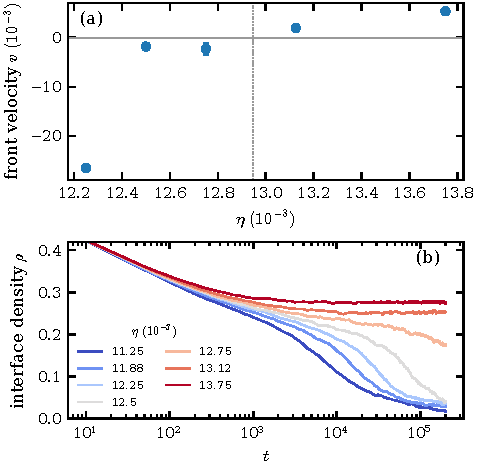
\includegraphics[width=\columnwidth]{figs/fig_eta}
\caption{The rule of Eq.~\eqref{eq:eta} at $\alpha = 1/2$. (a) Strip-front velocity against $\eta$
(three seeds; only fronts fitted over at least 20 records, since below $\eta^*$ the interior of the
strip nucleates the absorbing phase first); the dotted line is $\eta^* = 0.01295$. (b) Bulk interface
density against time at $L = 2048$.}
\label{fig:eta}
\end{figure}

\section{The five-cell rule of Molofsky \emph{et al.}: closure and simulation}
\label{app:molofsky}

\textit{Rule and closure.} The rule of Ref.~\cite{molofsky1999} is synchronous on the square
lattice, and a site's next state depends on the number $n$ of species-1 cells among the five
cells of its von Neumann neighborhood including itself: it becomes 1 with probability $p_n$,
where $p_0 = 0$, $p_5 = 1$, $p_3 = 1-p_2$, and $p_4 = 1-p_1$. In terms of the number $j$ of
disagreeing neighbors among the four, both states flip with probability $w(j) = p_j$, so the rule
is $\mathbb{Z}_2$-symmetric with two absorbing states, and its voter point is
$(p_1,p_2) = (1/5,2/5)$, where $w(j) = j/5$: the site copies one of the five cells, itself
included. Writing $w(j) = j/5 + g(j)$ gives $g = (0,\delta_1,\delta_2,-\delta_2,-\delta_1)$ with
$\delta_1 = p_1 - 1/5$ and $\delta_2 = p_2 - 2/5$. The dual of the voter point is a system of
five lazy coalescing walks, started at a site and its four neighbors, each staying with
probability $1/5$ or stepping to a neighbor with probability $1/5$; we sampled their lineage
patterns ($10^7$ samples per $T$) and evaluated the reaction function as in
Sec.~\ref{sec:theory}. Its structure is simpler than for the Moore neighborhood: with
$h(u) = u(1-u)(1-2u)$,
\begin{equation}
f(u) = h(u)\,[\,a + c\,u(1-u)\,],
\label{eq:fmol}
\end{equation}
with $a = \delta_1 a_1 + \delta_2 a_2$ and $c = P_5\,(10\,\delta_2 - 5\,\delta_1)$, where
$P_5(T)$ is the probability that all five lineages are distinct (the only five-class pattern,
which contributes exactly the mean-field map of Ref.~\cite{molofsky1999}) and $a_1$, $a_2$
collect the remaining patterns. Then $f'(0) = a$, $f'(1/2) = -(a + c/4)/2$, and
$\int_0^{1/2} f\,\ds u = (6a+c)/192$. Both $u = 0$ and $u = 1/2$ are stable, with the front
reversing in between, in the sector $-c/4 < a < 0$ of the $(\delta_1,\delta_2)$ plane, whose
angular width is set by $P_5$; the form~\eqref{eq:fmol} places the front reversal two thirds of
the way from the ray $f'(0) = 0$ to the ray $f'(1/2) = 0$. Because $c$ takes both signs as the
direction turns, every two-parameter rule has such a sector at finite $T$; the five-lineage
weight fixes its width, and its sign decides only whether a given one-parameter family, such as
$\kappa$ at fixed $\alpha$ for D\&N, crosses it.

Table~\ref{tab:molofsky} and Fig.~\ref{fig:molofsky}(a,b) give the closure's result. The sector
lies in the direction of small $p_1$ and large $p_2$, inside the mean-field multiple-outcome
wedge, around a line through the voter point of slope $\ds p_2/\ds p_1 = -3.46$ at $T = 65536$;
the empirical clustering--ergodic boundary of Ref.~\cite{molofsky1999}, which passes through
$(0.024, 1)$ and is described there by the dyad rule $3p_1 + p_2 = 1$, has slope $-3.4$ to $-3$
through the voter point. The window is $4.4^\circ$ wide at $T = 16$ and $0.45^\circ$ at
$T = 1024$, four to eight times narrower in relative terms than the D\&N window at the same $T$,
because five walks started on a plus stay distinct ten to forty times more rarely than nine
started on a $3\times3$ block. At the matching distance $\rho = 1/T$ from the voter point it is
about $5\times10^{-3}$ wide in $p$ at $T = 16$ and $5\times10^{-4}$ at $T = 64$. The search of
Ref.~\cite{molofsky1999}, at distances of order one from the voter point and with seeds of one
or two sites, could not have resolved it.

\begin{table}
\caption{The closure for the five-cell rule of Ref.~\cite{molofsky1999}: fraction of five-class
patterns among those with at least three classes, directions (degrees from the $+\delta_1$ axis)
of the rays $f'(0) = 0$ ($\theta_a$), $\int_0^{1/2} f = 0$ ($\theta_{\rm front}$), and
$f'(1/2) = 0$ ($\theta_{1/2}$), and the angular width of the bistable sector; $10^7$ samples per
$T$, bootstrap errors $\le 0.05^\circ$. Mean field ($T = 0$): $90^\circ$, $111.8^\circ$,
$123.7^\circ$, width $33.7^\circ$.}
\label{tab:molofsky}
\begin{ruledtabular}
\begin{tabular}{llllll}
$T$ & $P_5/P_{\ge3}$ & $\theta_a$ & $\theta_{\rm front}$ & $\theta_{1/2}$ & width \\
\hline
16 & 0.066 & 104.34 & 107.28 & 108.77 & 4.43 \\
64 & 0.025 & 105.32 & 106.60 & 107.25 & 1.92 \\
256 & 0.011 & 105.73 & 106.32 & 106.62 & 0.90 \\
1024 & 0.0052 & 105.93 & 106.23 & 106.38 & 0.45 \\
4096 & 0.0027 & 106.03 & 106.19 & 106.27 & 0.24 \\
65536 & 0.0008 & 106.09 & 106.14 & 106.17 & 0.07 \\
\end{tabular}
\end{ruledtabular}
\end{table}

\textit{Simulation.} We therefore simulated the rule itself, with the von Neumann neighborhood
added to the code of Appendix~\ref{app:numerics}, along two cuts across the predicted line,
$p_2 = 0.45$ and $0.50$, at distances $0.052$ and $0.104$ from the voter point. The protocol is
that of Sec.~\ref{sec:flagship}: planar fronts from a strip of the active phase ($L_x = 1024$--4096,
$L_y = 4096$, $6\times10^4$--$10^5$ steps, two to eight seeds, steps of $2.5\times10^{-4}$ in
$p_1$ near the reversal and of $10^{-4}$, down to $0.5\times10^{-4}$, within $3\times10^{-4}$ of
it), the mean population of $2\times2$ seeds ($2\times10^4$ replicas, $10^4$
steps), active disks of radius $R$ in the absorbing state (up to 400 replicas, $2\times10^4$
steps), and bulk runs from random initial conditions ($L = 256$--4096, $6\times10^4$--$1.2\times10^6$
steps, eight seeds at $L = 2048$ within $3\times10^{-4}$ of the line). At the voter point the mean population of a seed is conserved and the interface density
decays as $1/\ln t$, and at the three points on the edge $p_2 = 0$ described in
Ref.~\cite{molofsky1999} we reproduce their invasion, phase separation, and clustering.
Table~\ref{tab:molsim} and Fig.~\ref{fig:molofsky}(c) summarize the rest.

\begin{table}
\caption{Simulation of the five-cell rule of Ref.~\cite{molofsky1999} on the cuts $p_2 = 0.45$
and $0.50$ across the predicted line (distances $0.052$ and $0.104$ from the voter point),
against the closure of Table~\ref{tab:molofsky}. Directions are in degrees from the $+\delta_1$
axis; $p_1^*$ is the front reversal and $\Delta p_1 = p_1 - p_1^*$; ``seeds decay'' means that the mean population of a
$2\times2$ seed decreases over the first $10^2$--$10^3$ steps; $R_c$ is the radius at which an
active disk survives with probability $1/2$ at $2\times10^4$ steps; $\rho$ is the interface
density of the active phase. The active phase loses stability between the reversal and
$0.5\times10^{-4}$ above it, so the row for $|\theta_{1/2} - \theta_{\rm front}|$ is a bound.}
\label{tab:molsim}
\begin{ruledtabular}
\begin{tabular}{lll}
 & $p_2 = 0.45$ & $p_2 = 0.50$ \\
\hline
$p_1^*$ & $0.18535(3)$ & $0.17057(3)$ \\
$\theta_{\rm front}$ & $106.33$ & $106.40$ \\
\quad closure, $T = 16$, $1024$, $\infty$ & \multicolumn{2}{l}{$107.28$, $106.23$, $106.1$} \\
seeds decay for $\Delta p_1 <$ & $1.7\times10^{-3}$ & $2.4\times10^{-3}$ \\
\quad i.e. $\theta_a\approx$ & $104.5$ & $105.0$ \\
\quad closure, $T = 16$, $64$, $1024$ & \multicolumn{2}{l}{$104.34$, $105.32$, $105.93$} \\
$R_c v$ & $0.18$ & $0.16$--$0.19$ \\
active phase stable for $\Delta p_1\ge$ & $0.5\times10^{-4}$ & $0.5\times10^{-4}$ \\
\quad not stationary for $\Delta p_1\le$ & $0.4\times10^{-4}$ & $0$ \\
\quad i.e. $|\theta_{1/2} - \theta_{\rm front}|\le$ & $0.05$ & $0.03$ \\
\quad closure, $T = 16$, $64$, $1024$ & \multicolumn{2}{l}{$1.49$, $0.65$, $0.15$} \\
$\rho$ at $\Delta p_1 = 0.5\times10^{-4}$ & $0.188(1)$ & $0.20$ \\
$\rho$ at $\Delta p_1 = 1.5\times10^{-4}$ & $0.210(1)$ & $0.22$ \\
\end{tabular}
\end{ruledtabular}
\end{table}

\begin{figure}
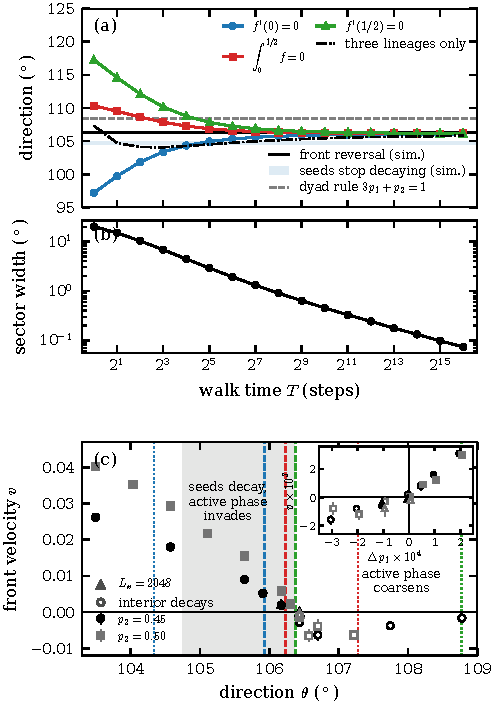
\includegraphics[width=\columnwidth]{figs/fig_molofsky}
\caption{The five-cell rule of Molofsky \emph{et al.}~\cite{molofsky1999}
(Appendix~\ref{app:molofsky}). (a) The closure: directions, in the plane $(\delta_1,\delta_2) =
(p_1-1/5,\,p_2-2/5)$ around the voter point, of the rays on which the absorbing state loses
linear stability, the front between the absorbing and the active state is stationary, and the
active state loses stability, against the walk time $T$; the bistable sector lies between the
first and the third. Solid line: the front reversal found by simulation,
$106.33^\circ$--$106.40^\circ$, which is also the direction of the chord from the voter point to
the boundary point $(0.024, 1)$ of Ref.~\cite{molofsky1999}; dashed line: their dyad rule
$3p_1+p_2 = 1$; band: where the mean population of a $2\times2$ seed stops decreasing in the
simulation. (b) Angular width of the sector. (c) The simulation: velocity of a planar front
(rows per step, positive when the active phase invades) against the direction $\theta$ on the
cuts $p_2 = 0.45$ (circles) and $0.50$ (squares); open symbols, the interior of the strip decays
during the run; triangles, $L_x = 2048$. Vertical lines: the closure's rays at $T = 16$ (dotted)
and $1024$ (dashed), colored as in (a). Shaded: the band in which the absorbing state is
metastable and the active phase invades. Inset: the crossing at steps of $10^{-4}$ in $p_1$
($L_x = 2048$ and, triangles, 4096; $L_y = 4096$, $10^5$ steps), against $\Delta p_1 = p_1 -
p_1^*$; the interior of the strip is stationary over the run (filled symbols) wherever $v > 0$
and decays (open) wherever $v\le0$.}
\label{fig:molofsky}
\end{figure}

The line is where the closure puts it. The front velocity is linear in $p_1$ through zero, with
slope $14$--$15$ at the reversal, at $p_1^* = 0.18535(3)$ and $0.17057(3)$ on the two cuts, the
error being the spread between three estimators of the velocity at $L_x = 2048$ and 4096. The
two reversals and the voter point are collinear, at $106.33^\circ$ and $106.40^\circ$ from the
$+\delta_1$ axis, slope $\ds p_2/\ds p_1 = -3.41(1)$ against the closure's $-3.46$;
extended, the line meets $p_2 = 1$ at $p_1 = 0.0235$, where Ref.~\cite{molofsky1999} places its
boundary point $(0.024, 1)$, and $p_2 = 0$ at $p_1 = 0.318$, between their phase separation at
$0.31$ and their invasion at $0.35$.

On the side where the active phase invades, the transition has the signatures of
Secs.~\ref{sec:bulk} and \ref{sec:drops}. The absorbing state is metastable: the mean population
of a $2\times2$ seed decreases for $p_1$ up to $1.5$--$2.5\times10^{-3}$ above $p_1^*$, i.e. up
to $\theta_a\approx 104.5^\circ$--$105^\circ$, as the closure gives for $T\approx 16$--$64$, the
seeds that survive to $10^4$ steps ($0.3$--$1.6\%$) being those that reached the critical radius;
and an active disk grows only beyond $R_c$, with $R_c v = 0.16$--$0.19$ at five points, i.e.
$R_c = D/v$ with $D = 1/5$ the diffusion constant of the lazy walk. The active phase is
stationary down to $0.5\times10^{-4}$ above $p_1^*$, where its interface density is $0.188(1)$
at $L = 2048$ and $0.190(1)$ at $L = 4096$. At $0.4\times10^{-4}$ it no longer settles, the
seeds wandering between $0.15$ and $0.19$ and $L = 4096$ drifting down to $0.176(3)$; at
$0.3\times10^{-4}$ it declines, and at $p_1^*$ it coarsens away. The density of the stationary
branch falls without a plateau from $0.30$ at $5\times10^{-3}$ above the line to $0.204(1)$ at
$10^{-4}$ and $0.188(1)$ at $0.5\times10^{-4}$, linearly in $\ln\Delta p_1$ at $0.021(5)$ per
$e$-fold, which $A/\ln(B/\Delta p_1)$, a power $\Delta p_1^{0.10}$, and a jump
$\rho_0 + C\,\Delta p_1^{0.3}$ with $\rho_0 = 0.14$ all reproduce with $p_1^*$ at the reversal
($\chi^2$ per degree of freedom $1.2$, $0.5$, $2.3$; a free $\rho_0$ stays below $0.12$ at two
standard deviations). But every continuous form anchored there predicts $0.18$ at the two points
below $0.5\times10^{-4}$, $0.01$--$0.03$ above what is measured, and with $p_1^*$ free every form
moves the line $1$--$4\times10^{-5}$ above the reversal, within its error and onto the stability
edge. So a logarithmic vanishing, as at a generalized voter transition, survives only with the
line $1$--$4\times10^{-5}$ above the reversal's central value, where the density $10^{-5}$ from
the line would still be $0.17$; telling that from a jump needs the line to better than
$10^{-5}$, and our data do not decide it. The band of absorbing-state metastability,
$1.5^\circ$--$2^\circ$ wide, is Case~4A of Ref.~\cite{cox2013} in two dimensions. It is what the
search of Ref.~\cite{molofsky1999} missed: it is narrower than the spacing of their parameter
scans, and inside it their seeds of one or two sites lie below $R_c$.

Across the line the two sides differ. The active phase has no metastable branch. At the
reversal and $1$--$3\times10^{-4}$ below it, its interface density declines from the start, only
slightly faster than the voter model's own $1/\ln t$, and the time to absorption grows with $L$,
by a factor $1.5$--$3.5$ from $L = 256$ to 512 (from $0.5$--$1.4\times10^5$ to
$1.1$--$2.0\times10^5$ steps below the line, and from $2.3$--$2.4\times10^5$ to
$4.6$--$8\times10^5$ at $p_1^*$ itself), as domains coarsen to the system size; the metastable
active phase of D\&N instead decays by nucleation after a plateau, with a lifetime independent
of $L$ [Fig.~\ref{fig:bulk}(c)]. Nowhere below the reversal does a stationary active slab
retreat: where $v < 0$ the strip dissolves in place, its interior at half of its early density
by $10^5$ steps already $10^{-4}$ below $p_1^*$, and wherever the interior is stationary,
$v > 0$ [Fig.~\ref{fig:molofsky}(c), inset]. The active phase thus loses stability within
$0.5\times10^{-4}$ of the reversal, i.e. within $0.05^\circ$ and $0.03^\circ$ on the two cuts,
and on the invading side of it if anywhere, where the closure puts the ray $f'(1/2) = 0$ beyond
the front by $1.5^\circ$ at $T = 16$, $0.65^\circ$ at $T = 64$, and $0.15^\circ$ at $T = 1024$.
For this rule the transition is thus first order on one side only: the absorbing state is
metastable where it loses, the active phase is not. The closure locates the line to $0.3^\circ$
and the absorbing-state branch of the window to the accuracy of its matching scale, and it
overstates the stability of the active phase beyond the reversal at every $T$ we computed; no
single $T$ fits the three rays, since $\theta_a$ wants $T\approx 16$--$64$, the natural
$T\sim 1/\rho$, the front is matched at $T\approx 300$, and the bound on $\theta_{1/2}$ needs
$T\gtrsim 10^4$. The caveats of Sec.~\ref{sec:theory} apply. Why the active-state branch is wide for D\&N, whose active phase is
metastable down to $0.9\,\qs$, and absent here, the closure does not explain; its
form~\eqref{eq:fmol}, with the reversal two thirds of the way across the window, is not what
the rule does.
\section{Numerical details}
\label{app:numerics}

\textit{Code.} The simulator stores 64 sites per 64-bit word. The eight neighbor bits of all sites
of a word are summed with bitwise adder trees, giving the number of live neighbors $k$ in four
bit planes; the flip class of each site is $(\sigma, k)$, with the flip probability $f_{\sigma k}$
read from an $2\times 9$ table, so that any outer-totalistic rule, Eq.~\eqref{eq:rule}, and the lazy
tables of Sec.~\ref{sec:async} are run by the same kernel. Each site draws one 32-bit uniform per
step from Philox$4\times32$-10~\cite{salmon2011} with counter (time, row, word, draw), and the 64
comparisons with the per-class thresholds are done bit-serially in parallel. Validation: (i) a
bit-exact comparison with a naive per-site implementation for five rules on four lattice shapes,
including one-word-wide and three-row lattices; (ii) per-class flip frequencies for an 18-class
table (variance of the $z$ scores over 560 repetitions $1.04\pm0.06$) and a $1.3\times10^8$-sample
test of the shared comparison on a voter-like table (per-class frequencies and adjacent-lane
independence, $|z|<2$); (iii) identical output for any number of threads and across restarts
from checkpoints; (iv) agreement with an independent GPU implementation of the $p = 0$ model to
1\% in the stationary density.

\textit{Replica mode.} For seeds and droplets, only the bounding box of the sites with a
disagreeing neighbor (plus a margin) is updated, refitted every 32 steps. This is exact because a
site with $j = 0$ cannot flip and its random numbers are indexed by position, not by the order
of updates; over 200 seeds, box and full-lattice updating give identical configurations at
every step. A replica whose box comes within 2 rows or 64 columns of the lattice edge is stopped
and counted as surviving. In the pure voter model the method reproduces the martingale
$\langle A(t)\rangle = 4$ for the number of live sites of a $2\times2$ seed (within $|z|<0.94$
at all 38 output times over $2\times10^5$ replicas) and $P_s(t)\propto\ln t/t$.

\textit{Front tracking.} For strip runs the per-row interface counts are smoothed over 32 rows;
each front is the first row, walking out from the strip center, where the smoothed density drops
below half the interior value $\iota_{\rm in}$ measured at $t = 10^3$. The velocity is fitted to
the strip width over the records with $t\ge 2000$, width between 15\% and 85\% of $L_y$, and the
strip center still active (density above $0.7\,\iota_{\rm in}$). Below $\qs$ the interior of a wide
strip eventually nucleates the absorbing phase; those records are excluded, which is why the
velocity is less precise below $\qs$ than above. Thresholds are the zero of the straight line
through the seed-averaged velocities at the two grid points that bracket the sign change. At
$p\ge 0.99$ (Table~\ref{tab:line}) the runs are $4\,t_\times$ long and the width is fitted for
$t\ge t_\times$ only; because holes open in the interior of a strip at coexistence before its
fronts have moved far, the width there is that of the outer envelope, the outermost row on either
side where the smoothed density exceeds $0.3\,\iota_{\rm in}$, which a hole cannot stop. The two
definitions agree to within $1.5\times10^{-5}$ in $\qs$ at $p = 0.99$ and 0.995. For the bands of
the orientation test (Sec.~\ref{sec:fronts}) the same outer-envelope tracking is applied to a
profile binned along the band normal, $s = (ay - bx)\bmod L$, which has $L$ bins of $L$ sites each
at a normal spacing of $1/\sqrt{a^2+b^2}$; the normal velocity is half the rate of change of the
band's normal width, fitted for $t\ge 10^4$, after the interior has relaxed, so that neither the
interior density nor its drift enters.

\textit{Droplets and holes.} In the two-droplet test (Sec.~\ref{sec:fronts}) the dead hole is cut
into a lattice that is random at $t = 0$ and relaxes to the active phase within $10^3$ steps. Since
the active phase has alive density $1/2$ by symmetry, the hole's chord in row $y$ is $L_x$ minus
twice the number of live sites in that row, and its area is the sum of the chords; the active
disk's area is twice its number of live sites. The radius $R = (A/\pi)^{1/2}$ is fitted for
$t\ge 10^4$.

\textit{Layer edges.} For the roughness of the wetting layer (Sec.~\ref{sec:wall}) full
configurations were stored every $10^5$ steps. In each column the two edges of the layer are its
lowest and highest interface sites within $L_y/4$ of the wall; their variances along the wall and
the height-difference correlation $\langle[h(x+r)-h(x)]^2\rangle$ give the roughness.

\textit{Cost.} About 2200 core hours in total, on Intel Xeon Platinum 8592+ nodes and a workstation,
at $(0.9$--$2.8)\times10^9$ site updates per second per core.

\bibliography{refs}

\end{document}
